\def\languageisfrench{}

\documentclass[a4paper,8pt]{extarticle} % extarticle allows to use font size of 8pt.

\usepackage[a4paper, top=1.6cm, bottom=2cm, left=1.6cm, right=1.6cm]{geometry} % Marge reduction.

%% Language specific package
\usepackage[french]{babel}
\frenchbsetup{StandardLists=true} % Necessary to use enumitem with babel/french.

%% Font and typing packages
\usepackage{fontspec}
\setmainfont[
	Ligatures=TeX,
	ItalicFont={Dancing Script},
	BoldItalicFont={Dancing Script}
	]{PT Serif} % default is Latin Modern
\newfontfamily\antiquefont[Ligatures=TeX]{Caslon Antique} % fancy font
\usepackage{microtype}			% Greatly improves general appearance of the text.
\usepackage{SIunits}			% Unit appearance.
\usepackage{xspace}				% Define commands that appear not to eat spaces.
\usepackage{ulem}				% To cross words out. Use \sout{}.

%% Array utilities
\usepackage{array}				% Additionnal options for arrays.
\usepackage{colortbl}			% Additionnal options for coloring arrays.
\usepackage[table]{xcolor}		% Auto alternate grey-white rows.
\usepackage[export]{adjustbox}		% Centered pics in tables

%% List utilities
\usepackage[inline]{enumitem}   % Display inline lists.
\usepackage{etoolbox}           % General utility. Good for lists for instance.
\usepackage{xparse}             % List utilities.
\usepackage{datatool}	% Handling alphabetical order.

%% Frames
\usepackage{framed}				% Boxes.
\usepackage[framemethod=TikZ]{mdframed}% For fancy frames.
\usepackage{tikz}				% For fancy frames.
\usepackage{wrapfig}			% Fancy insertion of pics in text.

%% Page utilities
\usepackage{multicol}			% Allows to divide a part of the page in multiple columns.
	
%% Others
\usepackage{keyval}             % Used to create maps of commands/labels/objects.
	\makeatletter                  % Mandatory for the usage of keyval.
\usepackage{xstring}            % String parsing, cutting, etc.
\usepackage{hyperref} % Links in PDF.


%%% Update of the dotfill command to always get dots

\newcommand{\predotfill}{\penalty0\hbox{}\nobreak}%


%%% Command to avoid typing \xspace when creating a new name macro

\newcommand{\newnamemacro}[2]{\newcommand{#1}{#2}} % \xspace removed for compatibility with alphabetical ordering

%%% Language specific stuff


\newcommand{\translationteam}{\item \og AEnoriel \fg \item \og Anglachel \fg \item \og Astadriel \fg \item \og Batcat \fg \item \og Bigfish \fg \item \og Eru \fg  \item \og Gandarin \fg \item \og Groumbahk \fg \item \og Iluvatar \fg \item \og Mammstein \fg \item \og Shlagrabak \fg \item et beaucoup d'autres...}

\hypersetup{
	pdfauthor={Équipe de traduction française de T9A},
	pdfsubject={Règles pour le jeu Batailles Fantastiques : Le 9\ieme{} Âge},
}

%%% Commands %%%

\ifdef{\isitanAB}{

\newcommand{\addtosortedlist}[1]{%
	\protected@edef\textarg{#1}%
	\protected@edef\textwithoutspaces{\expandafter\removespaces\expandafter{\textarg}}%
	\substitute\textwithoutspaces{É}{E}% Most used special characters of the language, and equivalent for alphabetical ordering
	\substitute\textwithoutspaces{È}{E}%
	\substitute\textwithoutspaces{Ê}{E}%
	\substitute\textwithoutspaces{é}{e}%
	\substitute\textwithoutspaces{è}{e}%
	\substitute\textwithoutspaces{ê}{e}%
	\substitute\textwithoutspaces{À}{A}%
	\substitute\textwithoutspaces{à}{a}%
	\substitute\textwithoutspaces{ù}{u}%
	\expandafter\sortitem\expandafter[\textwithoutspaces]{#1}%
}%

\newcommand{\pts}[1]{% First step is to remove spaces if there are some
	\def\numberwithoutspaces{\expandafter\removespaces\expandafter{#1}}%
	% Next step is getting rid of formatting if there are any (bold, color, ...)
	\pdfstringdef\cleannumber{\numberwithoutspaces}%
	% Now we can try if it is 1 or not
	\expandafter\ifstrequal\expandafter{\cleannumber}{1}{#1~\labels@point}{%
	\expandafter\ifstrequal\expandafter{\cleannumber}{0.5}{0,5~\labels@point}{%
	\expandafter\ifstrequal\expandafter{\cleannumber}{1.5}{1,5~\labels@point}{%
	#1~\labels@points}}}%
}

}{}

% Dark gods
\newcommand{\dchange}{Changement}
\newcommand{\dlust}{Luxure}
\newcommand{\pestilence}{Pestilence}
\newcommand{\wrath}{Courroux}
\newcommand{\truechaos}{Chaos Primordial}


% Nothing to edit here

\ifdef{\isitanAB}{

\newcommand{\alliancepts}[1]{
\ifsubstring{#1}{\free}{%
		\free{}%
	}{%
	\ifsubstring{#1}{\permodel}{%
		\splitatinf{#1}\myoption\myvalue%
		\pts{\myvalue}\permodel{}%
	}{%
	\pts{#1}
	}}
}

% You might wanna change the order of the gods - advanced user
\newcommand{\allianceoptions}[1]{%
	\defallianceoptions{#1}%
	\unitentryformat{\labels@allianceoptions\spacebeforecolon{}:}\newline
	\expandafter\ifblank\expandafter{\allianceoptions@introsentence}{}{\noindent\allianceoptions@introsentence{}\spacebeforecolon{}:}
	
	\expandafter\ifblank\expandafter{\allianceoptions@wrath}{
		\setlength{\columnseprule}{0.5pt}
		\renewcommand{\columnseprulecolor}{\color{black!30}}
		\vspace*{-0.2cm}\begin{multicols}{3}\raggedcolumns
		
			\begin{center}
			\noindent\dchange{}
			
			\noindent\alliancepts{\allianceoptions@change}
			\vspace*{-0.3cm}
			\end{center}
		
		\columnbreak
		
			\begin{center}
			\noindent\dlust{}
			
			\noindent\alliancepts{\allianceoptions@lust}
			\vspace*{-0.3cm}
			\end{center}
		
		\columnbreak

			\begin{center}
			\noindent\pestilence{}
			
			\noindent\alliancepts{\allianceoptions@pestilence}
			\vspace*{-0.3cm}
			\end{center}
			
		\end{multicols}
		\setlength{\columnseprule}{0pt}	
	}{
		\setlength{\columnseprule}{0.5pt}
		\renewcommand{\columnseprulecolor}{\color{black!30}}
		\vspace*{-0.2cm}\begin{multicols}{4}\raggedcolumns
		
			\begin{center}
			\noindent\dchange{}
			
			\noindent\alliancepts{\allianceoptions@change}
			\vspace*{-0.3cm}
			\end{center}
		
		\columnbreak

			\begin{center}
			\noindent\wrath{}
			
			\noindent\alliancepts{\allianceoptions@wrath}
			\vspace*{-0.3cm}
			\end{center}
		
		\columnbreak
		
			\begin{center}
			\noindent\dlust{}
			
			\noindent\alliancepts{\allianceoptions@lust}
			\vspace*{-0.3cm}
			\end{center}
		
		\columnbreak

			\begin{center}
			\noindent\pestilence{}
			
			\noindent\alliancepts{\allianceoptions@pestilence}
			\vspace*{-0.3cm}
			\end{center}
			
		\end{multicols}
		\setlength{\columnseprule}{0pt}
	}
}

}{}


%%% Labels %%%

% Profile

\newcommand{\labels@M}{M}
\newcommand{\labels@WS}{CC}
\newcommand{\labels@BS}{CT}
\newcommand{\labels@S}{F}
\newcommand{\labels@T}{E}
\newcommand{\labels@W}{PV}
\newcommand{\labels@I}{I}
\newcommand{\labels@A}{A}
\newcommand{\labels@Ld}{Cd}
\newcommand{\labels@Invocation}{Invocation} % For Vampire Covenant profiles
\newcommand{\labels@roundbase}{rond} % printed after XX mm for round bases

\newcommand{\Strength}{Force}

% Technical

\newcommand{\labels@range}{Portée}
\newcommand{\labels@point}{pt}
\newcommand{\labels@points}{pts}
\newcommand{\labels@only}{uniquement}
\newcommand{\labels@magic}{Magie}
\newcommand{\labels@pathsused}{Génère ses sorts dans la Discipline}
\newcommand{\labels@model}{figurine}
\newcommand{\labels@models}{figurines}
\newcommand{\labels@Singlemodel}{Figurine \textbf{seule}}

% Unit entry labels

\newcommand{\labels@basesize}{Socle}
\newcommand{\labels@trooptype}{Type de troupe}
\newcommand{\labels@specialrules}{Règles Spéciales}
\newcommand{\labels@alignment}{Allégeance}
\newcommand{\labels@alliance}{Allégeance}
\newcommand{\labels@allianceoptions}{Options d'Allégeance}
\newcommand{\labels@greenhiderace}{Race de Peaux Vertes}
\newcommand{\labels@equipment}{Équipement}
\newcommand{\labels@weapons}{Armes}
\newcommand{\labels@armour}{Armure}
\newcommand{\labels@options}{Options}
\newcommand{\labels@commandgroup}{État-Major}
\newcommand{\labels@charactermounts}{Montures de Personnages}
\newcommand{\labels@mounts}{Montures}
\newcommand{\labels@mount}{Monture}
\newcommand{\labels@specialequipment}{Équipement Spécial}

% Command groups

\newcommand{\labels@champion}{Champion}
\newcommand{\labels@standardbearer}{Porte-Étendard}
\newcommand{\labels@musician}{Musicien}
\newcommand{\labels@singlebannerallowance}{Une seule unité de ce type peut prendre une Bannière Magique}
\newcommand{\labels@condsinglebannerallowance}{Une seule unité de ce type peut prendre une Bannière Magique si}
\newcommand{\labels@bannerallowance}{Bannière Magique}
\newcommand{\labels@veteranstandardbearer}{Peut devenir Porte-Étendard Vétéran}
\newcommand{\labels@championallowance}{Arme Magique}

% Titles

\newcommand{\labels@armylist}{Liste des Troupes}
\newcommand{\labels@lords}{Seigneurs}
\newcommand{\labels@heroes}{Héros}
\newcommand{\labels@coreunits}{Unités de Base}
\newcommand{\labels@specialunits}{Unités Spéciales}
\newcommand{\labels@rareunits}{Unités Rares}
\newcommand{\labels@armywiderules}{Règles Communes de l'Armée}
\newcommand{\labels@armyspecialrules}{Règles Spéciales de l'Armée}
\newcommand{\labels@armoury}{Armurerie}
\newcommand{\labels@magicalitems}{Objets Magiques}
\newcommand{\labels@magicalweapons}{Armes Magiques}
\newcommand{\labels@magicalarmour}{Armures Magiques}
\newcommand{\labels@talismans}{Talismans}
\newcommand{\labels@enchanteditems}{Objets Enchantés}
\newcommand{\labels@arcaneitems}{Objets Cabalistiques}
\newcommand{\labels@magicalbanners}{Bannières Magiques}
\newcommand{\labels@quickrefsheet}{Fiche de Référence}
\newcommand{\labels@changelog}{Change Log}

\newcommand{\labels@lordsInitial}{S}
\newcommand{\labels@heroesInitial}{H}
\newcommand{\labels@coreunitsInitial}{B}
\newcommand{\labels@specialunitsInitial}{S}
\newcommand{\labels@rareunitsInitial}{R}
\newcommand{\labels@mountsInitial}{M}


% Titlepage

\newcommand{\labels@fantasybattles}{Batailles Fantastiques}
\newcommand{\labels@NinthAge}{Le 9\ieme{} Âge}
\newcommand{\labels@armyrules}{Règles de l'Armée}
\newcommand{\labels@frontpagecredits}{%
\labels@fantasybattles{} : \labels@NinthAge{} est un jeu créé et entretenu par la communauté qui met en scène des affrontements de figurines.\newline
Toutes les règles sont disponibles gratuitement sur le site suivant. Vos retours et suggestions sont les bienvenus : \url{http://www.the-ninth-age.com/}
}
\newcommand{\labels@license}{Copyright Creative Commons license : \url{the-ninth-age.com/license.html}}
\newcommand{\labels@tableofcontents}{Sommaire}
\newcommand{\labels@introduction}{%
\begin{center}\noindent{\Largerfontsize\textbf{Note des traducteurs}}\end{center}
\vspace{0.5cm}

Nous souhaitons remercier chaleureusement l'équipe à l'initiative du 9\ieme{} Âge pour leur motivation et leur travail continu pour faire vivre notre passion. Nous espérons que ce jeu saura développer les qualités pour plaire au plus grand nombre et réunir les joueurs, amateurs comme habitués des tournois, autour de règles amusantes et équilibrées, pour finalement s'imposer comme un standard du jeu de figurines. Une grande ambition qui ne pourra s'accomplir que \textbf{grâce à vous}, la communauté, via des retours constructifs, afin de modeler le jeu selon nos désirs. N'étant \textbf{en aucun cas à but lucratif}, le 9\ieme{} Âge part avec un avantage considérable. Les règles des éventuelles nouvelles sorties ne sont pas dictées par le besoin de vendre ces nouveautés. Vous pouvez choisir et acheter vos figurines où bon vous semble, il n'y a pas un unique revendeur toléré. Enfin, vous pouvez être assurés que tant que le 9\ieme{} Âge sera joué, vous disposerez d'un \textbf{support continu et régulier}, celui-ci étant offert par la communauté.

Concernant la traduction en elle-même, nous avons fait de notre mieux pour vous offrir une version de qualité, dont nous espérons qu'elle surpasse celle de la version originale ! Si vous constatez des coquilles, des erreurs, merci de nous les signaler en nous contactant sur le forum du 9\ieme{} Âge, dans le \textbf{sous-forum français} (\url{http://www.the-ninth-age.com/index.php?board/117-french/}). Vous y trouverez aussi les dernières mises à jour. \textbf{En cas de conflit d'interprétation avec la version originale, la version originale fait référence}.

\vspace{0.5cm}
Que ce jeu vous apporte d'innombrables heures de plaisir partagé !

\vspace{1cm}

\ifdef{\translationteam}{
	\begin{multicols}{3}
	\begin{itemize}
		\translationteam
	\end{itemize}
	\end{multicols}
}{}
}
\newcommand{\labels@rulechanges}{% blank ATM
}
\newcommand{\labels@latexcredit}{Document réalisé à l'aide de \LaTeX .}


%%% Technical commands

\newcommand{\only}[1]{(#1 uniquement)}
\newcommand{\free}{gratuit}
\newcommand{\upto}{jusqu'à}
\newcommand{\Upto}{Jusqu'à}
\newcommand{\unlimited}{pas de limite}
\newcommand{\permodel}{/fig.}
\newcommand{\listlastchoice}{ ou}
\newcommand{\notif}[1]{(pas #1)}
\newcommand{\wordand}{et}
\newcommand{\wordwith}{avec}
\newcommand{\ifNmodelsorless}[1]{(#1 figurines ou moins)}
\newcommand{\unitwith}{unité avec}
\newcommand{\From}{De} % From ... to ... models
\newcommand{\wordto}{à}
\newcommand{\wordAll}{Tous}
\newcommand{\spacebeforecolon}{ } % French put a space before colons
\newcommand{\minprice}{Coût min. :}
\newcommand{\mincostfor}{Coût min. pour}
\newcommand{\maxunitsize}{Taille max.}
\newcommand{\additionalfigscost}{Les figurines additionnelles coûtent}


%%% Special rules %%%

\newcommand{\ambush}{Embuscade}
\newcommand{\armourpiercing}[1]{Perforant\ifblank{#1}{}{ (#1)}}
\newcommand{\bodyguard}[1]{Garde du Corps\ifblank{#1}{}{ (#1)}}
\newcommand{\breathweapon}[1]{Attaque de Souffle\ifblank{#1}{}{ (#1)}}
\newcommand{\channel}{Canalisation}
\newcommand{\crushattack}{Attaque Écrasante}
\newcommand{\daemonicinstability}{Instabilité Démoniaque}
\newcommand{\devastatingcharge}{Charge Dévastatrice}
\newcommand{\distracting}{Distrayant}
\newcommand{\divineattacks}{Attaques Divines}
\newcommand{\engineer}{Ingénieur}
\newcommand{\ethereal}{Éthéré}
\newcommand{\fastcavalry}{Cavalerie Légère}
\newcommand{\fear}{Peur}
\newcommand{\fightinextrarank}{Combat avec un Rang Supplémentaire}
\newcommand{\fireborn}{Né du Feu}
\newcommand{\flamingattacks}{Attaques Enflammées}
\newcommand{\flammable}{Inflammable}
\newcommand{\frenzy}{Frénésie}
\newcommand{\fly}[1]{Vol\ifblank{#1}{}{ (#1)}}
\newcommand{\grindingattacks}[1]{Attaques de Broyage\ifblank{#1}{}{ (#1)}}
\newcommand{\hardtarget}{Camouflé}
\newcommand{\hatred}{Haine}
\newcommand{\hellfire}{Feu Démoniaque}
\newcommand{\hidden}{Caché}
\newcommand{\holyattacks}{Attaques Divines} % deprecated, still has to be filled. same as Divine Attacks.
\newcommand{\immunetopsychology}{Immunisé à la Psychologie}
\newcommand{\impacthits}[1]{Touches d'Impact\ifblank{#1}{}{ (#1)}}
\newcommand{\insignificant}{Insignifiant}
\newcommand{\largetarget}{Grande Cible}
\newcommand{\lethalstrike}{Coup Fatal}
\newcommand{\lightningattacks}{Attaques Foudroyantes}
\newcommand{\lightningreflexes}{Réflexes Foudroyants}
\newcommand{\lighttroops}{Troupe Légère}
\newcommand{\magicresistance}[1]{Résistance à la Magie\ifblank{#1}{}{ (#1)}}
\newcommand{\magicalattacks}{Attaques Magiques}
\newcommand{\metalshifting}{Fusion du Métal}
\newcommand{\moveorfire}{Mouvement ou Tir}
\newcommand{\multipleshots}[1]{Tirs Multiples\ifblank{#1}{}{ (#1)}}
\newcommand{\multiplewounds}[2]{Blessures Multiples\ifblank{#1}{}{ (#1\ifblank{#2}{)}{, #2)}}}
\newcommand{\notaleader}{Pas un Meneur}
\newcommand{\otherworldly}{D'Outre-Monde}
\newcommand{\pathmaster}[1]{Maître de la Voie\ifblank{#1}{}{ (#1)}}
\newcommand{\poisonedattacks}{Attaques Empoisonnées}
\newcommand{\quicktofire}{Tir Rapide}
\newcommand{\randommovement}[1]{Mouvement Aléatoire\ifblank{#1}{}{ (#1)}}
\newcommand{\randomattacks}[1]{Attaques Aléatoires\ifblank{#1}{}{ (#1)}}
\newcommand{\regeneration}[1]{Régénération\ifblank{#1}{}{ (#1+)}}
\newcommand{\reload}{Rechargez !}
\newcommand{\requirestwohands}{Arme à deux Mains}
\newcommand{\scythes}{Faux}
\newcommand{\scout}{Éclaireur}
\newcommand{\scouts}{Éclaireurs}
\newcommand{\stomp}[1]{Piétinement\ifblank{#1}{}{ (#1)}}
\newcommand{\strider}[1]{Guide\ifblank{#1}{}{ (#1)}}
\newcommand{\stubborn}{Tenace}
\newcommand{\stupidity}{Stupidité}
\newcommand{\skirmisher}{Tirailleur}
\newcommand{\skirmishers}{Tirailleurs}
\newcommand{\sweepingattack}{Attaque au Passage}
\newcommand{\swiftstride}{Course Rapide}
\newcommand{\thunderouscharge}{Charge Tonitruante}
\newcommand{\terror}{Terreur}
\newcommand{\toxicattacks}{Attaques Toxiques}
\newcommand{\unbreakable}{Indémoralisable}
\newcommand{\undead}{Mort-Vivant}
\newcommand{\unstable}{Instable}
\newcommand{\unwieldy}{Encombrant}
\newcommand{\vanguard}{Avant-Garde}
\newcommand{\volleyfire}{Tir de Volée}
\newcommand{\warplatform}{Plateforme de Guerre}
\newcommand{\wardsave}[1]{Sauvegarde Invulnérable\ifblank{#1}{}{ (#1+)}}
\newcommand{\weaponmaster}{Maître d'Ar\-mes}
\newcommand{\wizardconclave}[1]{Conclave de Sorciers\ifblank{#1}{}{ (#1)}}


%%% Magic %%%


% General

\newcommand{\Pathof}{Voie}

\newcommand{\battle}{Commune}

\newcommand{\anyofthebattlemagic}{dans n'importe laquelle des Voies Communes}
\newcommand{\ONLYanyofthebattlemagic}{Commune de votre choix}

\newcommand{\magiclevel}[1]{\ifnumcomp{#1}{<}{3}{Apprenti Magicien}{Maître Magicien} Niveau #1}
\newcommand{\Level}{Niveau}

\newcommand{\wizard}{Magicien}
\newcommand{\wizards}{Magiciens}

\newcommand{\learnedspell}{Sort Appris}
\newcommand{\learnedspells}{Sorts Appris}
\newcommand{\attributespell}{Attribut de la Voie}
\newcommand{\attributespells}{Attributs de la Voie}
\newcommand{\attributespellnumber}{A}
\newcommand{\traitspell}{Sort Caractéristique}
\newcommand{\traitspells}{Sorts Caractéristiques}
\newcommand{\traitspellnumber}{C}


\newcommand{\boundspell}[1]{Objet de Sort\ifblank{#1}{}{, Puissance #1}}
\newcommand{\boundspells}[1]{Objets de Sort\ifblank{#1}{}{, Puissance #1}}

% Casting Vocabulary

\newcommand{\lostfocus}{Perte de Concentration}
\newcommand{\miscast}{Fiasco}
\newcommand{\miscasts}{Fiascos}
\newcommand{\overwhelmingpower}{Pouvoir Irrésistible}

\newcommand{\breachintheveil}{Brèche dans le Voile}
\newcommand{\catastrophicdetonation}{Explosion Catastrophique}
\newcommand{\witchfire}{Feu de Sorcières}
\newcommand{\sorcerousbacklash}{Contrecoup Magique}
\newcommand{\amnesia}{Amnésie}

% Spell Types

\newcommand{\augment}{Amélioration}
\newcommand{\hex}{Malédiction}
\newcommand{\universal}{Universel}
\newcommand{\missile}{Projectile}
\newcommand{\damage}{Dégâts}
\newcommand{\direct}{Direct}
\newcommand{\focused}{Focalisé}
\newcommand{\vortex}{Vortex}
\newcommand{\ground}{Marqueur}
\newcommand{\linetemplate}{Gabarit de Ligne}
\newcommand{\specialTYPE}{Spécial}
\newcommand{\aura}{Aura}
\newcommand{\castersunit}{Unité du Lanceur}
\newcommand{\caster}{Lanceur}

\newcommand{\template}{Gabarit}

% Spell Durations

\newcommand{\lastsoneturn}{Dure un Tour}
\newcommand{\instant}{Immédiat}
\newcommand{\permanent}{Permanent}
\newcommand{\remainsinplay}{Reste en Jeu}


% Battle Magic

\newcommand{\alchemy}{de l'Alchimie}
\newcommand{\alchemyattribute}{Édit de Fer}
\newcommand{\alchemysignature}{Métal Fondu}
\newcommand{\alchemyspellone}{Lames Enchantées}
\newcommand{\alchemyspelltwo}{Corrosion Rampante}
\newcommand{\alchemyspellthree}{Manteau de Vif-Argent}
\newcommand{\alchemyspellfour}{Pieu d'Argent}
\newcommand{\alchemyspellfive}{Fléau de l'Acier}
\newcommand{\alchemyspellsix}{Transmutation en Or}

\newcommand{\death}{de la Mort}
\newcommand{\deathattribute}{Nuage de Désespoir}
\newcommand{\deathsignature}{Le Baiser de la Faucheuse}
\newcommand{\deathspellone}{Malédiction du Mortel}
\newcommand{\deathspelltwo}{Esprits Dévorants}
\newcommand{\deathspellthree}{Sangsue Psychique}
\newcommand{\deathspellfour}{Moisson d’Âmes}
\newcommand{\deathspellfive}{L’Abîme aussi te Regarde...}
\newcommand{\deathspellsix}{Maelström d’Âmes}

\newcommand{\fire}{du Feu}
\newcommand{\fireattribute}{Feu Déchaîné}
\newcommand{\firesignature}{Boule de Feu}
\newcommand{\firespellone}{Cascade Ardente}
\newcommand{\firespelltwo}{Épées Flamboyantes}
\newcommand{\firespellthree}{Jet de Flammes}
\newcommand{\firespellfour}{Traits Enflammés}
\newcommand{\firespellfive}{Remparts Incandescents}
\newcommand{\firespellsix}{Souffler sur les Braises}

\newcommand{\heavens}{des Cieux}
\newcommand{\heavensattribute}{Second Sceau}
\newcommand{\heavenssignature}{Aquilon}
\newcommand{\heavensspellone}{Bourrasque}
\newcommand{\heavensspelltwo}{Choc Foudroyant}
\newcommand{\heavensspellthree}{Conjonction Astrale}
\newcommand{\heavensspellfour}{Fléau du Ponant}
\newcommand{\heavensspellfive}{Déluge d'Éclairs}
\newcommand{\heavensspellsix}{Appel de la Comète}

\newcommand{\light}{de la Lumière}
\newcommand{\lightattribute}{Lumière Gardienne}
\newcommand{\lightsignature}{Éclat Brûlant}
\newcommand{\lightspellone}{Bouclier Protecteur}
\newcommand{\lightspelltwo}{Étincelle de Courage}
\newcommand{\lightspellthree}{Vitesse Fulgurante}
\newcommand{\lightspellfour}{Toile Scintillante}
\newcommand{\lightspellfive}{Distorsion Temporelle}
\newcommand{\lightspellsix}{Bannissement Divin}

\newcommand{\nature}{de la Nature}
\newcommand{\natureattribute}{Souffle de Vie}
\newcommand{\naturesignature}{Eaux Vivifiantes}
\newcommand{\naturespellone}{Maître de la Terre}
\newcommand{\naturespelltwo}{Le Trône de Chêne}
\newcommand{\naturespellthree}{Esprits des Bois}
\newcommand{\naturespellfour}{Croissance Estivale}
\newcommand{\naturespellfive}{Peau Rocailleuse}
\newcommand{\naturespellsix}{Créatures Souterraines}

\newcommand{\shadows}{des Ombres}
\newcommand{\shadowsattribute}{Course Parmi les Ombres}
\newcommand{\shadowssignature}{Miasmes Obscurs}
\newcommand{\shadowsspellone}{Orbe de Noirceur}
\newcommand{\shadowsspelltwo}{Partir en Fumée}
\newcommand{\shadowsspellthree}{Expérience de Mort Imminente}
\newcommand{\shadowsspellfour}{Char Vaporeux}
\newcommand{\shadowsspellfive}{Ombres Dévorantes}
\newcommand{\shadowsspellsix}{Scalpel Psychique}

\newcommand{\wilderness}{de la Sauvagerie}
\newcommand{\wildernessattribute}{La Chasse Sauvage}
\newcommand{\wildernesssignature}{La Bête qui Sommeille}
\newcommand{\wildernessspellone}{Essaim d’Insectes}
\newcommand{\wildernessspelltwo}{Rage Intérieure}
\newcommand{\wildernessspellthree}{Pieu de Rougebois}
\newcommand{\wildernessspellfour}{Calamité des Bois Sauvages}
\newcommand{\wildernessspellfive}{Tempête Furieuse}
\newcommand{\wildernessspellsix}{Métamorphose
Monstrueuse}

\newcommand{\eightpaths}{Octuple}



% Army Specific Magic

\newcommand{\butchery}{de la Boucherie}
\newcommand{\butcheryattribute}{Sang de Kholag}
\newcommand{\butcherysignature}{Briseur de Dents}
\newcommand{\butcheryspellone}{Buveur de Moelle}
\newcommand{\butcheryspelltwo}{Festin de Tripaille}
\newcommand{\butcheryspellthree}{Concasseur d’Os}
\newcommand{\butcheryspellfour}{Gobeur de Cervelle}
\newcommand{\butcheryspellfive}{Cœur de Troll}
\newcommand{\butcheryspellsix}{Gosier de Géant}

\newcommand{\change}{du Changement}
\newcommand{\changeattribute}{Vent du Changement}
\newcommand{\changesignature}{Feu Azur}
\newcommand{\changespellone}{Feu Rose}
\newcommand{\changespelltwo}{Vague du Changement}
\newcommand{\changespellthree}{Secrets Volés}
\newcommand{\changespellfour}{Règne de la Confusion}
\newcommand{\changespellfive}{Inéluctable Trahison}
\newcommand{\changespellsix}{Portail Éternel}

\newcommand{\thebiggreengods}{des Grands Dieux Verts}
\newcommand{\thebiggreengodsattribute}{Chopez-les !}
\newcommand{\thebiggreengodssignature}{L'Heure de la Raclée}
\newcommand{\thebiggreengodsspellone}{Coup de Boule}
\newcommand{\thebiggreengodsspelltwo}{Poings Bastonneurs}
\newcommand{\thebiggreengodsspellthree}{Même Pas Mal !}
\newcommand{\thebiggreengodsspellfour}{Grande Main Verte}
\newcommand{\thebiggreengodsspellfive}{Boum !}
\newcommand{\thebiggreengodsspellsix}{Le Gros Piétinement}

\newcommand{\thelittlegreengods}{des Petits Dieux Verts}
\newcommand{\thelittlegreengodsattribute}{Fourbe Larcin}
\newcommand{\thelittlegreengodssignature}{Œil Mauvais}
\newcommand{\thelittlegreengodsspellone}{Taillades Sournoises}
\newcommand{\thelittlegreengodsspelltwo}{Bénédiction de la Mère-Araignée}
\newcommand{\thelittlegreengodsspellthree}{Ça Démange ?}
\newcommand{\thelittlegreengodsspellfour}{Chut ! Pas un Bruit...}
\newcommand{\thelittlegreengodsspellfive}{J’vous Arrange Ça}
\newcommand{\thelittlegreengodsspellsix}{Malédiction de la Lune Verte}

\newcommand{\blackmagic}{de la Magie Noire}
\newcommand{\blackmagicattribute}{Soif d’Âmes}
\newcommand{\blackmagicsignature}{Furie de Moraec}
\newcommand{\blackmagicspellone}{Rafale Glaciale}
\newcommand{\blackmagicspelltwo}{Tourbillon de Lames}
\newcommand{\blackmagicspellthree}{Agonie Paralysante}
\newcommand{\blackmagicspellfour}{Marque de la Peur}
\newcommand{\blackmagicspellfive}{Trait d’Énergie Noire}
\newcommand{\blackmagicspellsix}{Terreur Noire}

\newcommand{\disease}{de la Maladie}
\newcommand{\diseaseattribute}{Bénédiction Nécrotique}
\newcommand{\diseasesignature}{Relents de Pestilence}
\newcommand{\diseasespellone}{Haleine Corruptrice}
\newcommand{\diseasespelltwo}{Toucher Putréfiant}
\newcommand{\diseasespellthree}{Excroissance Adipeuse}
\newcommand{\diseasespellfour}{Purge Parasitaire}
\newcommand{\diseasespellfive}{Malédiction du Lépreux}
\newcommand{\diseasespellsix}{Tourbillon Fétide}

\newcommand{\lust}{de la Luxure}
\newcommand{\lustattribute}{Masochisme}
\newcommand{\lustsignature}{Flagellation Démoniaque}
\newcommand{\lustspellone}{Grâce Hypnotique}
\newcommand{\lustspelltwo}{Valse Irrésistible}
\newcommand{\lustspellthree}{Hystérie}
\newcommand{\lustspellfour}{Fantasmagorie}
\newcommand{\lustspellfive}{Déchirement psychique}
\newcommand{\lustspellsix}{Chœur Dissonant}

\newcommand{\necromancy}{de la Nécromancie}
\newcommand{\necromancyattribute}{Tromper la Faucheuse}
\newcommand{\necromancysignature}{Adjuration des Morts}
\newcommand{\necromancyspellone}{Parodie de Vie}
\newcommand{\necromancyspelltwo}{Convocation Profanatoire}
\newcommand{\necromancyspellthree}{Sarabande Macabre}
\newcommand{\necromancyspellfour}{Regard de Setesh}
\newcommand{\necromancyspellfive}{Vol de Jeunesse}
\newcommand{\necromancyspellsix}{Malédiction des Morts}

\newcommand{\ruin}{de la Ruine}
\newcommand{\ruinattribute}{Hordes Sans Fin}
\newcommand{\ruinsignature}{Éclair Noir}
\newcommand{\ruinspellone}{Nourrissons-les...}
\newcommand{\ruinspelltwo}{Souiller le Sol}
\newcommand{\ruinspellthree}{La Faim}
\newcommand{\ruinspellfour}{Appel de la Tempête}
\newcommand{\ruinspellfive}{Rupture Sismique}
\newcommand{\ruinspellsix}{Pour Qui Sonne le Glas}

\newcommand{\forge}{de la Forge}
\newcommand{\forgeattribute}{Fournaise Haineuse}
\newcommand{\forgesignature}{Bouclier de Sombrefeu}
\newcommand{\forgespellone}{Rage Incendiaire}
\newcommand{\forgespelltwo}{Subjugation}
\newcommand{\forgespellthree}{Souffle de Haine}
\newcommand{\forgespellfour}{Anathème de Noirceur}
\newcommand{\forgespellfive}{Cendres Asphyxiantes}
\newcommand{\forgespellsix}{Flammes de la Forge}

\newcommand{\sands}{des Sables}
\newcommand{\sandsattribute}{Les Morts sans Repos}
\newcommand{\sandssignature}{Sirocco}
\newcommand{\sandsspellone}{Lames Maudites}
\newcommand{\sandsspelltwo}{Dessiccation Mortelle}
\newcommand{\sandsspellthree}{Frappes Vengeresses}
\newcommand{\sandsspellfour}{Jugement Divin}
\newcommand{\sandsspellfive}{Sables Mouvants}
\newcommand{\sandsspellsix}{Écho des Gloires
Passées}

\newcommand{\whitemagic}{de la Magie Blanche}
\newcommand{\whitemagicattribute}{Bouclier des Anciens}
\newcommand{\whitemagicsignature}{Traits de Lumière}
\newcommand{\whitemagicspellone}{Résurrection du Phénix}
\newcommand{\whitemagicspelltwo}{Volonté Inspirante}
\newcommand{\whitemagicspellthree}{Sentier Secret}
\newcommand{\whitemagicspellfour}{Bénédiction d’Amhar}
\newcommand{\whitemagicspellfive}{Fusion d’Artefact}
\newcommand{\whitemagicspellsix}{Cataclysme}

% Paths Initials

\newcommand{\alchemyInitials}{A}
\newcommand{\deathInitials}{M}
\newcommand{\fireInitials}{F}
\newcommand{\heavensInitials}{C}
\newcommand{\lightInitials}{L}
\newcommand{\natureInitials}{N}
\newcommand{\shadowsInitials}{O}
\newcommand{\wildernessInitials}{S}

\newcommand{\eightfoldInitials}{8}

\newcommand{\whitemagicInitials}{MB}
\newcommand{\blackmagicInitials}{MN}
\newcommand{\necromancyInitials}{N}
\newcommand{\sandsInitials}{S}
\newcommand{\forgeInitials}{F}
\newcommand{\biggreengodsInitials}{GDV}
\newcommand{\littlegreengodsInitials}{PDV}
\newcommand{\butcheryInitials}{B}
\newcommand{\ruinInitials}{R}
\newcommand{\diseaseInitials}{M}
\newcommand{\lustInitials}{L}
\newcommand{\changeInitials}{C}


%%% Other rules %%%

% Troop types rules

\newcommand{\combinedprofile}{Profil Combiné}
\newcommand{\cavalrysupport}{Soutien de Cavalerie}
\newcommand{\monstrousranks}{Rangs Monstrueux}
\newcommand{\monstroussupport}{Soutien Monstrueux}
\newcommand{\monsterranks}{Rang de Monstre}

\newcommand{\armoursave}{Sauvegarde d'Armure}
\newcommand{\frontrank}{Au Premier Rang}
\newcommand{\hardcover}{Couvert Lourd}
\newcommand{\holdyourground}{Tenez les Rangs}
\newcommand{\inspiringpresence}{Présence Charismatique}
\newcommand{\lightcover}{Couvert Léger}
\newcommand{\ordnance}{Artillerie}
\newcommand{\parry}{Parade}
\newcommand{\raisewounds}{Ressusciter des Figurines}
\newcommand{\recoverwounds}{Récupérer des PVs}
\newcommand{\rnf}{ordinaires}
\newcommand{\general}{Général}
\newcommand{\bsb}{Porteur de la Grande Bannière}
\newcommand{\cannotmarch}{Pas de Marche Forcée}
\newcommand{\veteranstandardbearer}{Porte-Étendard Vétéran}
\newcommand{\swirlingmelee}{Mêlée Tourbillonnante}
\newcommand{\scoringunit}{Unité de Capture}
\newcommand{\scoringunits}{Unités de Capture}


%%% Equipment %%%

\newcommand{\hw}{Arme de Base}
\newcommand{\pw}{Paire d'Armes}
\newcommand{\spear}{Lance}
\newcommand{\halberd}{Hallebarde}
\newcommand{\gw}{Arme Lourde}
\newcommand{\lance}{Lance de Cavalerie}
\newcommand{\lightlance}{Lance Légère}
\newcommand{\flail}{Fléau}

\newcommand{\throwingweapons}{Armes de Jet}
\newcommand{\shortbow}{Arc Court}
\newcommand{\bow}{Arc}
\newcommand{\longbow}{Arc Long}
\newcommand{\handgun}{Arquebuse}
\newcommand{\crossbow}{Arbalète}
\newcommand{\pistol}{Pistolet}
\newcommand{\braceofpistols}{Paire de Pistolets}	

\newcommand{\innatedefence}[1]{Protection Innée\ifblank{#1}{}{~(#1+)}}
\newcommand{\mountsprotection}[1]{Protection de Monture\ifblank{#1}{}{~(#1+)}}
\newcommand{\la}{Armure Légère}
\newcommand{\ha}{Armure Lourde}
\newcommand{\platearmour}{Armure de Plates}
\newcommand{\shield}{Bouclier}
\newcommand{\barding}{Caparaçon}

\newcommand{\cannon}{Canon}
\newcommand{\cannons}{Canons}
\newcommand{\catapult}{Catapulte}
\newcommand{\catapults}{Catapultes}
\newcommand{\volleygun}{Batterie de Tir}
\newcommand{\boltthrower}{Baliste}
\newcommand{\flamethrower}{Lance-Flammes}
\newcommand{\artilleryweapon}{Arme d'Artillerie}


%%% Troop types %%%

\newcommand{\characters}{Personnages}
\newcommand{\infantry}{Infanterie}
\newcommand{\monstrousinfantry}{Infanterie Monstrueuse}
\newcommand{\cavalry}{Cavalerie}
\newcommand{\monstrouscavalry}{Cavalerie Monstrueuse}
\newcommand{\swarm}{Nuée}
\newcommand{\swarms}{Nuées}
\newcommand{\warbeast}{Bête de Guerre}
\newcommand{\warbeasts}{Bêtes de Guerre}
\newcommand{\monster}{Monstre}
\newcommand{\monsters}{Monstres}
\newcommand{\monstrousbeast}{Bête Monstrueuse}
\newcommand{\monstrousbeasts}{Bêtes Monstrueuses}
\newcommand{\chariot}{Char}
\newcommand{\chariots}{Chars}
\newcommand{\riddenmonster}{Monstre Monté}
\newcommand{\riddenmonsters}{Monstres Montés}
\newcommand{\warmachine}{Machine de Guerre}
\newcommand{\warmachines}{Machines de Guerre}


%%% Terrain %%%

\newcommand{\water}{Eaux Peu Profondes}
\newcommand{\forest}{Forêt}
\newcommand{\impassableterrain}{Terrain Infranchissable}


%%% Profile wording

\newcommand{\oneperarmy}{Un par Armée}
\newcommand{\oneofakind}{Uni\-que}
\newcommand{\zerotoXchoice}[1]{0-#1 Choix}
\newcommand{\onechoiceonlyNOC}{(un seul choix)}
\newcommand{\onfootonly}{(à pied uniquement)}
\newcommand{\closecombatonly}{seulement au Corps à Corps}
\newcommand{\Xmodelsorless}[1]{(max. #1 figurines)}
\newcommand{\magicalitemsallowance}{Objets Magiques}
\newcommand{\magicalweaponallowance}{Arme Magique}
\newcommand{\notmagicalarmour}{(pas d'Armure Magique)}
\newcommand{\weapononechoice}{\optionschoice{Arme \onechoiceonlyNOC{} :}}
\newcommand{\weaponschoice}{\optionschoice{Armes :}}
\newcommand{\shootingweapononechoice}{\optionschoice{Arme de Tir \onechoiceonlyNOC{} :}}
\newcommand{\combatweapononechoice}{\optionschoice{Arme de Corps à Corps \onechoiceonlyNOC{} :}}
\newcommand{\combatweapononechoiceTWOCOL}{\optionschoiceTWOCOL{Arme de Corps à Corps \onechoiceonlyNOC{} :}}
\newcommand{\armouronechoice}{\optionschoice{Armure \onechoiceonlyNOC{} :}}
\newcommand{\magiclevelchoice}{\optionschoice{Magie \onechoiceonlyNOC{} :}}
\newcommand{\mustbecomeoneofthefollowing}{\optionschoice{\textbf{Doit} devenir au choix :}}
\newcommand{\mustbecomeoneofthefollowingNOC}{Doit devenir au choix :}
\newcommand{\musttakeoneormoreofthefollowing}{\optionschoice{\textbf{Doit} prendre au moins un choix :}}
\newcommand{\musttakeoneofthefollowing}{\optionschoice{\textbf{Doit} prendre un et un seul choix :}}
\newcommand{\musttakeoneofthefollowingNOC}{Doit choisir entre :}
\newcommand{\uptotwoofthefollowing}{\optionschoice{Jusqu'à deux choix :}}
\newcommand{\uptotwoofthefollowingTWOCOL}{\optionschoiceTWOCOL{Jusqu'à deux choix :}}

\newcommand{\onechoiceonly}{\optionschoice{Un seul choix :}}
\newcommand{\onechoiceonlyTWOCOL}{\optionschoiceTWOCOL{Un seul choix :}}

\newcommand{\maytake}{Peut prendre}




%%% Orcs N Goblins debug, let it as it is

\newcommand{\pershadygit}{debug}
\newcommand{\permadgit}{debug}

%%% Dwarven Holds debug, let it as it is

\newcommand{\perrune}{debug}


%%% Commands to handle strings, better than xstring to handle commands inside the strings %%%

\newcommand{\substitute}[3]{%
  \protected@edef\sub@temp{#1}%
  \saveexpandmode
  \expandarg\StrSubstitute{\sub@temp}{#2}{#3}[#1]%
  \restoreexpandmode
}

\newcommand{\splitatstar}[3]{%
  \protected@edef\split@temp{#1}%
  \saveexpandmode
  \expandarg\StrCut{\split@temp}{*}#2#3%
  \restoreexpandmode
}

\newcommand{\splitatinf}[3]{%
  \protected@edef\split@temp{#1}%
  \saveexpandmode
  \expandarg\StrCut{\split@temp}{<}#2#3%
  \restoreexpandmode
}

\newcommand{\splitatequal}[3]{%
  \protected@edef\split@temp{#1}%
  \saveexpandmode
  \expandarg\StrCut{\split@temp}{=}#2#3%
  \restoreexpandmode
}

\newcommand{\ifsubstring}[4]{%
  \protected@edef\split@temp{#1}%
  \protected@edef\split@tempbis{#2}%
  \saveexpandmode
  \expandarg\IfSubStr{\split@temp}{\split@tempbis}{#3}{#4}%
  \restoreexpandmode
}

\def\removespaces#1{\zap@space#1 \@empty}

%%% Commands for alphabetical ordering %%%

\newcommand{\sortitem}[2][\relax]{%
	\DTLnewrow{list}% Create a new entry
	\ifx#1\relax%
		\DTLnewdbentry{list}{sortlabel}{#2}% Add entry sortlabel (no optional argument)
	\else%
		\DTLnewdbentry{list}{sortlabel}{#1}% Add entry sortlabel (optional argument)
	\fi%
		\DTLnewdbentry{list}{description}{#2}% Add entry description
}
\newenvironment{sortedlist}{%
	\DTLifdbexists{list}{\DTLcleardb{list}}{\DTLnewdb{list}}% Create new/discard old list
}{%
	\DTLsort{sortlabel}{list}% Sort list
	\begin{itemize*}[label={}, itemjoin={,}]%
		\DTLforeach*{list}{\theDesc=description}{%
		\item\theDesc}% Print each item
	\end{itemize*}%
}

\pdfstringdefDisableCommands{\def\textcolor#1{}}

% See language specific file for \addtosortedlist

%%% Database for automatic Quick Ref Sheet %%%

\DTLnewdb{profiles} % Database containing name, category, multiprofile number, profilename (if multi), caraclist, trooptype, invocation for CV.
\newcommand{\profilecategory}{\labels@lords} % Will be updated in relevant categories

\newcommand{\profiledtbfillname}[1]{\DTLnewdbentry{profiles}{name}{#1}}
\newcommand{\profiledtbfillcategory}[1]{\DTLnewdbentry{profiles}{category}{#1}}
\newcommand{\profiledtbfilltrooptype}[1]{\DTLnewdbentry{profiles}{trooptype}{#1}}
\newcommand{\profiledtbfillinvocation}[1]{\DTLnewdbentry{profiles}{invocation}{#1}}
\newcommand{\profiledtbfillprofile}[1]{\DTLnewdbentry{profiles}{profile}{#1}}
\newcommand{\profiledtbfillmultipleprofile}[1]{\DTLnewdbentry{profiles}{multipleprofile}{#1}}

\newcommand{\void}[1]{}
\newcounter{multiprofilecounter}

\newcommand{\profiledtbfillcarac}[1]{%
	\profiledtbfillprofile{#1}
	\parselist{#1}{\locallists@profileslist}% Split of the different profiles in the case of a multiprofile.
	\setcounter{multiprofilecounter}{0}%
	\forlistloop{\stepcounter{multiprofilecounter}\void}{\locallists@profileslist}%
	\expandafter\profiledtbfillmultipleprofile\expandafter{\number\value{multiprofilecounter}}
}


%%% Technical commands %%%

\newcommand{\newrule}{\textcolor{green!50!black}}
\newcommand{\removedrule}[1]{\textcolor{green!50!black}{\sout{#1}}}
\newcommand{\starsymbol}{$\star$}
\newcommand{\refsymbol}{$^\star$}

\newcommand{\inch}{\arcsecond}
\newcommand{\foot}{\arcminute}
\newcommand{\range}[1] {\labels@range~\unit{#1}{\inch}}
\newcommand{\distance}[1] {\unit{#1}{\inch}}
\newcommand{\result}[1] {\texttt{'}#1\texttt{'}}
\newcommand{\plusone}{+1}


%%% Fonts and sizes %%%

\newcommand{\bigtitle}[1]{\vspace*{-1.5cm}\section*{}\noindent\begin{center}\Hugefontsize\textbf{\antiquefont\expandafter\uppercase\expandafter{#1}}\end{center}}

\newcommand{\subtitle}[1]{\subsection*{}\noindent{\hugefontsize\antiquefont #1}}

\newcommand{\subsubtitle}[1]{\subsubsection*{}\noindent{\Largerfontsize\antiquefont #1}}

\newcommand{\verysmallfontsize}{\fontsize{4}{4.8}\selectfont}
\newcommand{\smallfontsize}{\fontsize{6}{7.2}\selectfont}
\newcommand{\normalfontsize}{\fontsize{8}{9.6}\selectfont}
\newcommand{\largefontsize}{\fontsize{10}{12}\selectfont}
\newcommand{\largerfontsize}{\fontsize{12}{14.4}\selectfont}
\newcommand{\Largefontsize}{\fontsize{14}{16.8}\selectfont}
\newcommand{\Largerfontsize}{\fontsize{15}{18}\selectfont}
\newcommand{\hugefontsize}{\fontsize{18}{21.6}\selectfont}
\newcommand{\Hugefontsize}{\fontsize{25}{30}\selectfont}

\newcommand{\unitentryformat}[1]{\textit{\largefontsize{#1}}}
\newcommand{\textIT}[1]{\textit{\largefontsize{#1}}}


%%% Titles %%%

\newcommand{\lordstitle}{\def\logolocalpath{../Layout/pics/logo_lord.png}\bigtitle{\labels@lords}}
\newcommand{\heroestitle}{%
\def\logolocalpath{../Layout/pics/logo_hero.png}%
\clearpage\bigtitle{\labels@heroes}%
\renewcommand{\profilecategory}{\labels@heroes}%
}
\newcommand{\coreunitstitle}{%
\def\logolocalpath{../Layout/pics/logo_core.png}%
\clearpage\bigtitle{\labels@coreunits}%
\renewcommand{\profilecategory}{\labels@coreunits}%
}
\newcommand{\specialunitstitle}{%
\def\logolocalpath{../Layout/pics/logo_special.png}%
\clearpage\bigtitle{\labels@specialunits}%
\renewcommand{\profilecategory}{\labels@specialunits}%
}
\newcommand{\rareunitstitle}{%
\def\logolocalpath{../Layout/pics/logo_rare.png}%
\clearpage\bigtitle{\labels@rareunits}%
\renewcommand{\profilecategory}{\labels@rareunits}%
}
\newcommand{\mountstitle}{%
\def\logolocalpath{../Layout/pics/logo_mount.png}%
\clearpage\bigtitle{\labels@charactermounts}%
\renewcommand{\profilecategory}{\labels@mounts}%
}

\newcommand{\startarmywiderules}{\newpage\bigtitle{\labels@armywiderules}\largefontsize}
\newcommand{\closearmywiderules}{\normalfontsize}
\newcommand{\armywideruleentry}[1]{\subtitle{#1}\vspace{5pt}}

\newcommand{\startarmyspecialrules}{\bigtitle{\labels@armyspecialrules}\largefontsize}
\newcommand{\closearmyspecialrules}{\normalfontsize}
\newcommand{\armyspecialruleentry}[1]{\subtitle{#1}\vspace{5pt}}

\newcommand{\startarmyarmoury}{\bigtitle{\labels@armoury}\largefontsize\subtitle{}}
\newcommand{\closearmyarmoury}{\normalfontsize}

\newcommand{\startarmymagicalitems}{\newpage\largefontsize\bigtitle{\labels@magicalitems}\begin{multicols}{2}\raggedcolumns}
\newcommand{\closearmymagicalitems}{\end{multicols}\normalfontsize}

\newcommand{\armymagicalweapons}{\subtitle{\labels@magicalweapons}}
\newcommand{\armymagicalarmour}{\subtitle{\labels@magicalarmour}}
\newcommand{\armytalismans}{\subtitle{\labels@talismans}}
\newcommand{\armyenchanteditems}{\subtitle{\labels@enchanteditems}}
\newcommand{\armyarcaneitems}{\subtitle{\labels@arcaneitems}}
\newcommand{\armymagicalbanners}{\subtitle{\labels@magicalbanners}}

\newcommand{\startarmynewsection}[1]{\newpage\bigtitle{#1}\largefontsize}
\newcommand{\startarmynewsectionSP}[1]{\vspace{1.5cm}\bigtitle{#1}\largefontsize}
\newcommand{\closearmynewsection}{\normalfontsize}

\newcommand{\armynewsubsection}[1]{\subtitle{#1}\vspace{5pt}}
\newcommand{\armynewsubsubsection}[1]{\subsubtitle{#1}\vspace{3pt}}

\newcommand{\armylist}{\clearpage}

\newcommand{\quickrefsheettitle}{\clearpage\newgeometry{top=1.6cm, bottom=2cm, left=1cm, right=1cm}\bigtitle{\labels@quickrefsheet}\vspace*{0.4cm}}
\newcommand{\changelogtitle}{\clearpage\bigtitle{\labels@changelog}\spaceaftersection{}}

\newcommand{\spaceaftersection}{\vspace{0.8cm}}

\newcommand{\separator}{\noindent\begin{center}\textcolor{black!30}{\rule{0.7\columnwidth}{2pt}}\end{center}}


%%% Custom lists and description for first sections of the army books

\newcommand{\startpricelist}{\begin{samepage}\begin{description}[leftmargin=0.3cm, labelindent=0cm, labelsep=0.1cm]}
\def\endpricelist{\end{description}\end{samepage}}
\newcommand{\pricelistitem}[2]{\item \option{\textbf{#1}}{#2}\newline}
\newcommand{\nopricelistitem}[1]{\item \textbf{#1}\newline}

\newcommand{\startpricelistNSP}{\begin{description}[leftmargin=0.3cm, labelindent=0cm, labelsep=0.1cm]}
\def\endpricelistNSP{\end{description}}

\newcommand{\startitemlist}{\begin{multicols}{2}\raggedcolumns\begin{description}[leftmargin=0.3cm, labelindent=0cm, labelsep=0.1cm]}
\def\enditemlist{\end{description}\end{multicols}}
\newcommand{\listitem}[1]{\item[#1\spacebeforecolon{}:]}

\newcommand{\startitemlistonecol}{\begin{description}[leftmargin=0.3cm, labelindent=0cm, labelsep=0.1cm]}
\def\enditemlistonecol{\end{description}}
\newcommand{\listitemonecol}[1]{\item \textbf{#1\spacebeforecolon{}:}\newline}

\newenvironment{customitemize}{\begin{description}[leftmargin=0.3cm, labelindent=0cm, labelsep=0cm]}{\end{description}}
\newenvironment{customsubitemize}{\begin{itemize}[label={-}, labelsep=0.1cm, topsep=0cm, parsep=0cm, itemsep=0cm, leftmargin=0.4cm, labelindent=0cm]}{\end{itemize}}

%%% Table parameters %%%

\newcolumntype{M}[1]{>{\centering\let\newline\\\arraybackslash\hspace{0pt}}m{#1}}


%%%  Lists handling %%%

\newcommand{\addlocallist}{\listadd\locallists@dummy}%
\NewDocumentCommand{\parsespacelist}{>{\SplitList{ }} m }{%
	\ProcessList{#1}{\addlocallist}%
}%
\NewDocumentCommand{\parsecommalist}{>{\SplitList{,}} m }{%
	\ProcessList{#1}{\addlocallist}%
}%
\newcommand{\parselist}[3][,]{%
	\renewcommand\addlocallist{\listadd#3}%
  	\undef#3%
  	\ifstrequal{#1}{ }{\parsespacelist{#2}}{\parsecommalist{#2}}%
}


%%% Profiles handling %%%

% Element of a table that contains the characteristics of a model (or part of a model)
\newcommand\caraclist[1]{
	\parselist[ ]{#1}{\locallists@caraclist}%
	\forlistloop{&}{\locallists@caraclist}%
}

\newcommand\caraclistbold[1]{
	\parselist[ ]{#1}{\locallists@caraclist}%
	\forlistloop{&\bfseries}{\locallists@caraclist}%
}

% Line of a profile table, including bottom line. It is meant to contain the name of the model (or part), its characteristics (preferably, the second argument should contain the \carac macro), troop type and base size.
\newcommand{\profilefirstline}[4]{#1 & #2 &   & #3 & #4 }

% Start of a profile table. Includes the table commands, and the column labels. \profilecellsize is the size of the characteristics cells in the profile.
\newcommand{\profilecellsize}{0.56cm}
\newcommand{\profilestart}{%
	\noindent %
	\begin{tabular}{@{}p{3cm}@{}M{\profilecellsize}@{}M{\profilecellsize}@{}M{\profilecellsize}@{}M{\profilecellsize}@{}M{\profilecellsize}@{}M{\profilecellsize}@{}M{\profilecellsize}@{}M{\profilecellsize}@{}M{\profilecellsize}@{}p{2.7cm}@{}p{3.3cm}@{}p{2cm}@{}}%
	 &% \textbf{\labels@profile}
	\labels@M & \labels@WS & \labels@BS & \labels@S & \labels@T & \labels@W & \labels@I & \labels@A & \labels@Ld &%
	&%
	{\unitentryformat{\labels@trooptype}} &%
	{\unitentryformat{\labels@basesize}}%
}

% End of a profile table.
\newcommand{\profileend}{\end{tabular}}

% Algorithm to automatically use and fill previous command, with coherence check.
\providebool{profilefirst}
\newcommand{\profileitem}[1]{%
	\tabularnewline%
	\splitatinf{#1}\local@unitname\local@unitprofile%
	\local@unitname \expandafter\caraclistbold\expandafter{\local@unitprofile}%
	&%
	& \ifbool{profilefirst}{\unit@type}{}%
	& \ifbool{profilefirst}{%
		\ifsubstring{\unit@basesize}{x}{% Rectangular base
			\unit{\unit@basesize}{\milli\meter}%
		}{% Circular base
			\unit{\unit@basesize}{\milli\meter} \labels@roundbase%
		}%
	}{}%
	\global\boolfalse{profilefirst}%
}
\newcommand{\profile}[1]{%
	\parselist{#1}{\locallists@profileslist}%
	\profilestart%
	\global\booltrue{profilefirst}%
	\forlistloop{\profileitem}{\locallists@profileslist}%
	\profileend%
}


%%% Profiles handling in case of invocation %%%

\newcommand{\invocprofilestart}{%
	\noindent %
	\begin{tabular}{@{}p{3cm}@{}M{\profilecellsize}@{}M{\profilecellsize}@{}M{\profilecellsize}@{}M{\profilecellsize}@{}M{\profilecellsize}@{}M{\profilecellsize}@{}M{\profilecellsize}@{}M{\profilecellsize}@{}M{\profilecellsize}@{}M{2.2cm}@{}p{0.5cm}@{}p{3.3cm}@{}p{2cm}@{}}%
	 &% \textbf{\labels@profile}
	\labels@M & \labels@WS & \labels@BS & \labels@S & \labels@T & \labels@W & \labels@I & \labels@A & \labels@Ld & \unitentryformat{\labels@Invocation} &%
	&%
	{\unitentryformat{\labels@trooptype}} &%
	{\unitentryformat{\labels@basesize}}%
}

\newcommand{\invocprofileitem}[1]{%
	\tabularnewline%
	\splitatinf{#1}\local@unitname\local@unitprofile%
	\local@unitname \expandafter\caraclistbold\expandafter{\local@unitprofile}%
	& \ifbool{profilefirst}{\unit@invocation}{} &%
	& \ifbool{profilefirst}{\unit@type}{}%
	& \ifbool{profilefirst}{\unit{\unit@basesize}{\milli\meter}}{}%
	\global\boolfalse{profilefirst}%
}

\newcommand{\invocprofile}[1]{%
	\parselist{#1}{\locallists@profileslist}%
	\invocprofilestart%
	\global\booltrue{profilefirst}%
	\forlistloop{\invocprofileitem}{\locallists@profileslist}%
	\profileend%
}


%%%%%%%%%%%%%%%%%%
%%% Unit rules %%%
%%%%%%%%%%%%%%%%%%

%%% Entry title command %%%

\newcommand{\unitentry}[2]{\ifdefempty{#1}{}{\noindent #2}}


%%% Special rules %%%

% Special rules listing for a unit, with alphabetical order.
\newcommand{\ruleslist}[1]{%
	\parselist[,]{#1}{\locallists@ruleslist}%
	\begin{sortedlist}%
		\forlistloop{\addtosortedlist}{\locallists@ruleslist}%
	\end{sortedlist}%
}

% Special rules entry.
\newcommand{\specialrules}[1]{\unitentry{#1}{\unitentryformat{\labels@specialrules\spacebeforecolon{}:}\newline\hspace*{-\fontdimen2\font}\expandafter\ruleslist\expandafter{#1}.}}
\newcommand{\commonspecialrules}[2]{\unitentry{#2}{\unitentryformat{#1\spacebeforecolon{}:}\newline\hspace*{-\fontdimen2\font}\expandafter\ruleslist\expandafter{#2}.}}


%%% Magical abilities %%%

% Paths listing for a unit.
\newcommand{\pathslist}[1]{%
	\parselist[,]{#1}{\locallists@pathslist}%
	\begin{itemize*}[label={}, itemjoin={,}, itemjoin*={\listlastchoice}]%
		\forlistloop{\item}{\locallists@pathslist}%
	\end{itemize*}%
}

% Magic entry.
\newcommand{\magic}[2]{\unitentry{#2}{\unitentryformat{\labels@magic\spacebeforecolon{}: }\newline\ifdefempty{#1}{}{\textbf{\magiclevel{#1}}. }\labels@pathsused\expandafter\pathslist\expandafter{#2}.}}

% Wizard Conclave.
\newcommand{\magicwizardconclave}[1]{\unitentry{#1}{\unitentryformat{\labels@magic\spacebeforecolon{}: }\newline\textbf{\wizardconclave{}}\spacebeforecolon{}: #1.}}


%%% Equipment %%%

% Equipment listing.
\newcommand{\equipmentlist}[1]{%
	\parselist[,]{#1}{\locallists@equipmentlist}%
	\begin{sortedlist}%
		\forlistloop{\addtosortedlist}{\locallists@equipmentlist}%
	\end{sortedlist}%
}

% Equipment entry.
\newcommand{\weapons}[1]{\unitentry{#1}{\unitentryformat{\labels@weapons\spacebeforecolon{}:}\newline\hspace*{-\fontdimen2\font}\expandafter\equipmentlist\expandafter{#1}.}}

\newcommand{\armour}[1]{\unitentry{#1}{\unitentryformat{\labels@armour\spacebeforecolon{}:}\newline\hspace*{-\fontdimen2\font}\expandafter\equipmentlist\expandafter{#1}.}}


%%% Alignment %%%

\newcommand{\alignment}[1]{\unitentry{#1}{\unitentryformat{\labels@alignment\spacebeforecolon{}:}\newline\textbf{#1}.}}

%%% Green Hide Race %%%

\newcommand{\greenhideraceentry}[1]{\unitentry{#1}{\unitentryformat{\labels@greenhiderace\spacebeforecolon{}:}\newline\textbf{#1}.}}


%%% Options %%%

% Frame commands.
\newcommand{\optionsframestart}{\begin{innerframe}[\labels@options]}
\newcommand{\optionsframeend}{\end{innerframe}}

% Options listing.
\newcommand{\optionslist}[1]{%
	\parselist[,]{#1}{\locallists@optionslist}%
	\begin{description}[leftmargin=0.3cm, labelindent=0cm, labelsep=0cm, itemsep=0cm, parsep=0cm]%
		\forlistloop{\item\setoption}{\locallists@optionslist}%
	\end{description}%
}

% Options entry.
\newcommand{\options}[1]{\ifdefempty{#1}{}{\optionsframestart\vspace*{-0.4cm}\unitentry{#1}{\expandafter\optionslist\expandafter{#1}}\optionsframeend}}

% Option specific commands.
\newcommand{\setoption}[1]{%
	\noexpandarg\StrCut{#1}{=}\optiontext\optionvalue%
	\expandafter\ifstrequal\expandafter{\optionvalue}{}{%
		\optiontext%
	}{%
	\ifsubstring{\optionvalue}{\free}{%
		\option[\free]{\optiontext}{\optionvalue}%
	}{%
	\ifsubstring{\optionvalue}{\unlimited}{%
		\option[\unlimited]{\optiontext}{\optionvalue}%
	}{%
	\ifsubstring{\optionvalue}{\upto}{%
		\splitatinf{\optionvalue}\myoption\myvalue%
		\option[\upto]{\optiontext}{\myvalue}%
	}{%
	\ifsubstring{\optionvalue}{\permodel}{%
		\splitatinf{\optionvalue}\myoption\myvalue%
		\option[\permodel]{\optiontext}{\myvalue}%
	}{%
	\ifsubstring{\optionvalue}{\pershadygit}{% For Orcs N Goblins
		\splitatinf{\optionvalue}\myoption\myvalue%
		\option[\pershadygit]{\optiontext}{\myvalue}%
	}{%
	\ifsubstring{\optionvalue}{\permadgit}{% For Orcs N Goblins
		\splitatinf{\optionvalue}\myoption\myvalue%
		\option[\permadgit]{\optiontext}{\myvalue}%
	}{%	
	\ifsubstring{\optionvalue}{\perrune}{% For Dwarven Holds
		\splitatinf{\optionvalue}\myoption\myvalue%
		\option[\perrune]{\optiontext}{\myvalue}%
	}{%	
		\option{\optiontext}{\optionvalue}%
	}}}}}}}}%
}

\newcommand{\option}[3][]{#2\predotfill\dotfill\nobreak%
	% Add \upto token if necessary.
	\ifstrequal{#1}{\upto}{\upto~}{}%
	% The option can be free, have an unlimited cost, or have a points cost.
	\ifstrequal{#1}{\free}{\free}{\ifstrequal{#1}{\unlimited}{\unlimited}{\pts{#3}}}%
	% Add \permodel if necessary.
	\ifstrequal{#1}{\permodel}{\nobreak\permodel}{}%
	% Add \persomething if necessary.
	\ifstrequal{#1}{\pershadygit}{\nobreak\pershadygit}{}% For Orcs N Goblins
	\ifstrequal{#1}{\permadgit}{\nobreak\permadgit}{}% For Orcs N Goblins
	\ifstrequal{#1}{\perrune}{\nobreak\perrune}{}% For Dwarven Holds
}

\newcommand\optionschoice[2]{%
	\parselist[,]{#2}{\locallists@optionschoice}%
	#1%
	\begin{itemize}[label={}, parsep=0cm, labelindent=0cm, labelwidth=0cm, noitemsep, topsep=0em, leftmargin=0.3cm]%
	\forlistloop{\item\setoption}{\locallists@optionschoice}%
	\end{itemize}%
}

\newcommand\optionschoiceTWOCOL[2]{%
	\parselist[,]{#2}{\locallists@optionschoice}%
	#1%
	\begin{itemize}[label={}, parsep=0cm, labelindent=0cm, labelwidth=0cm, noitemsep, topsep=0em, leftmargin=0.3cm]%
	\setlength{\columnseprule}{0.5pt}
	\renewcommand{\columnseprulecolor}{\color{black!30}}
	\vspace*{-5pt}\begin{multicols}{2}\raggedcolumns
	\forlistloop{\item\setoption}{\locallists@optionschoice}%
	\end{multicols}\setlength{\columnseprule}{0pt}
	\end{itemize}%
}

% Option description in army desc.
\newcommand{\optiondef}[3]{\option{\textbf{#1}}{#2}\ifblank{#3}{}{\\{#3}}}


%%% Mount options %%%

% Frame commands.
\newcommand{\mountsframestart}{\begin{innerframe}[\labels@mounts]}
\newcommand{\mountsframeend}{\end{innerframe}}

% Mount listing.
\newcommand{\mountslist}[1]{%
	\parselist[,]{#1}{\locallists@mountslist}%
	\begin{description}[leftmargin=0.3cm, labelindent=0cm, labelsep=0cm, itemsep=0cm, parsep=0cm]%
		\forlistloop{\item\setoption}{\locallists@mountslist}%
	\end{description}%
}

% Mount entry.
\newcommand{\mounts}[1]{\ifdefempty{#1}{}{\mountsframestart\vspace*{-0.4cm}\unitentry{#1}{\expandafter\mountslist\expandafter{#1}}\mountsframeend}}


%%% Command group %%%

% Command group specific commands.
\define@key{commandgroup}{restriction}            {\def\commandgroup@restriction{#1}}
\define@key{commandgroup}{champion}               {\def\commandgroup@champion{#1}}
\define@key{commandgroup}{championallowance}      {\def\commandgroup@championallowance{#1}}
\define@key{commandgroup}{championoption}         {\def\commandgroup@championoption{#1}}
\define@key{commandgroup}{championprerestriction} {\def\commandgroup@championprerestriction{#1}}
\define@key{commandgroup}{championrestriction}    {\def\commandgroup@championrestriction{#1}}
\define@key{commandgroup}{banner}                 {\def\commandgroup@banner{#1}}
\define@key{commandgroup}{bannerallowance}        {\def\commandgroup@bannerallowance{#1}}
\define@key{commandgroup}{veteranstandardbearer}  {\def\commandgroup@veteranstandardbearer{#1}}
\define@key{commandgroup}{singlebannerallowance}  {\def\commandgroup@singlebannerallowance{#1}}
\define@key{commandgroup}{condsinglebannerallowance}  {\def\commandgroup@condsinglebannerallowance{#1}}
\define@key{commandgroup}{banneroption}           {\def\commandgroup@banneroption{#1}}
\define@key{commandgroup}{bannerrestriction}      {\def\commandgroup@bannerrestriction{#1}}
\define@key{commandgroup}{musician}               {\def\commandgroup@musician{#1}}
\define@key{commandgroup}{musicianrestriction}    {\def\commandgroup@musicianrestriction{#1}}
\newcommand{\defcommandgroup}{%
	\setkeys{commandgroup}{restriction=,
	                       champion=, championallowance=, championoption=, championprerestriction=, 
	                       championrestriction=, banner=, bannerallowance=, veteranstandardbearer=, 
	                       singlebannerallowance=, condsinglebannerallowance=, banneroption=, 
	                       bannerrestriction=, musician=, musicianrestriction=}%
	\setkeys{commandgroup}%
}

% Frame commands.
\newcommand{\commandgroupframestart}{\begin{innerframe}[\labels@commandgroup]}
\newcommand{\commandgroupframeend}{\end{innerframe}}

% Command group entry.
\newcommand{\commandgroup}[1]{%
	\defcommandgroup{#1}%
	\ifstrempty{#1}{}{\commandgroupframestart\vspace*{-0.2cm}%
		\begin{description}[leftmargin=0.3cm, labelindent=0cm, labelsep=0cm, itemsep=0cm, parsep=0cm]%
			% Command group title, including restrictions applying to all the command group
			\item \textbf{\expandafter\ifblank\expandafter{\commandgroup@restriction}{}{ \only{\commandgroup@restriction}\spacebeforecolon{}: }} 
			% Champion handling.
			\ifdefempty{\commandgroup@champion}{}{% We have a champion!
			\ifdefempty{\commandgroup@championprerestriction}{% There is no prerestriction to have a champion
				\item \hspace*{-0.04cm}\option{\labels@champion%
					% Possible restrictions to taking a champion
				    \expandafter\ifblank\expandafter{\commandgroup@championrestriction}{}{ \only{\commandgroup@championrestriction}}%
				    % Cost of a champion
				    }{\commandgroup@champion}%
				    % Magical allowance of the champion. Should probably not be used, champion option can do it as well and is more flexible.
					\ifdefempty{\commandgroup@championallowance}{}{\par\option[\upto]{\hspace*{0.3cm}- \labels@championallowance}{\commandgroup@championallowance}}%
					% Any option available to the champion, in the form option:cost
					\ifdefempty{\commandgroup@championoption}{}{%
						\splitatinf{\commandgroup@championoption}\local@option\local@cost%
						\par\option{\hspace*{0.3cm}- \local@option}{\local@cost}}%
			}{% There is a pre-restriction to have a champion
				\item \hspace*{-0.04cm}\commandgroup@championprerestriction	\newline%
				\option{\labels@champion}{\commandgroup@champion}%
				% Magical allowance of the champion. Should probably not be used, champion option can do it as well and is more flexible.
				\ifdefempty{\commandgroup@championallowance}{}{\par\option[\upto]{\hspace*{0.3cm}- \labels@championallowance}{\commandgroup@championallowance}}%
				% Any option available to the champion, in the form option:cost
				\ifdefempty{\commandgroup@championoption}{}{%
					\splitatinf{\commandgroup@championoption}\local@option\local@cost%
					\par\option{\hspace*{0.3cm}- \local@option}{\local@cost}}%
			} %End of the prerestriction of not condition
			}% End of champion handling
			\ifdefempty{\commandgroup@musician}{}{% We have a musician!
				\item \hspace*{-0.04cm}\option{\labels@musician%
					% Possible restrictions to taking a musician
				    \expandafter\ifblank\expandafter{\commandgroup@musicianrestriction}{}{ \only{\commandgroup@musicianrestriction}}%
				    % Cost of a musician
				    }{\commandgroup@musician}%
			}%
			\ifdefempty{\commandgroup@banner}{}{% We have a banner!
				\item \hspace*{-0.04cm}\option{\labels@standardbearer%
					% Possible restrictions to taking a banner
				    \expandafter\ifblank\expandafter{\commandgroup@bannerrestriction}{}{ \only{\commandgroup@bannerrestriction}}%
				    % Cost of a banner
				    }{\commandgroup@banner}%
				    % Magical banner, if all units of this type can take one.
					\ifdefempty{\commandgroup@bannerallowance}{}{\par\option[\upto]{\hspace*{0.3cm}- \labels@bannerallowance}{\commandgroup@bannerallowance}}%
					% Magical banner, if Veteran.
					\ifdefempty{\commandgroup@veteranstandardbearer}{}{\par\hspace*{0.3cm}- \labels@veteranstandardbearer%
					\expandafter\ifstrequal\expandafter{\commandgroup@veteranstandardbearer}{*}{*}{}%
					}%
					% Magical banner, if only one unit of this type can take one.
					\ifdefempty{\commandgroup@singlebannerallowance}{}{\par\option[\upto]{\hspace*{0.3cm}- \labels@singlebannerallowance}{\commandgroup@singlebannerallowance}}%
					% Magical banner, if only one unit of this type can take one, but with condtions.
					\ifdefempty{\commandgroup@condsinglebannerallowance}{}{%
						\splitatinf{\commandgroup@condsinglebannerallowance}\local@option\local@cost%
						\par\option[\upto]{\hspace*{0.3cm}- \labels@condsinglebannerallowance \local@option}{\local@cost}}%
					% Additional option for the banner, such as Hill Goblin Lookouts for Ogres
					\ifdefempty{\commandgroup@banneroption}{}{%
						\splitatinf{\commandgroup@banneroption}{\local@option}{\local@cost}%
						\par\option{\hspace*{0.3cm}- \local@option}{\local@cost}%
					}%
			}%
		\end{description}%
	\commandgroupframeend%
	 }%
}


%%% Unit rules %%%

% Frame commands.
\newcommand{\unitrulesframestart}{\begin{innerframe}[\labels@specialrules]}
\newcommand{\unitrulesframeend}{\end{innerframe}}

% Unit rules specific commands.
\newcommand{\unitrule}[2]{\item[#1\spacebeforecolon{}:]#2}

% Unit rule entry.
\newcommand{\unitrules}[1]{\ifdefempty{#1}{}{\unitrulesframestart\vspace*{-0.05cm}\begin{description}[leftmargin=0.3cm, labelindent=0cm, labelsep=0.1cm, itemsep=0.2cm, parsep=0cm]#1\end{description}\unitrulesframeend}}


%%% Special equipment %%%

% Frame commands.
\newcommand{\unitequipmentframestart}{\begin{innerframe}[\labels@specialequipment]}
\newcommand{\unitequipmentframeend}{\end{innerframe}}

% Special equipment specific commands.
\newcommand{\equipmentdef}[2]{\item[#1\spacebeforecolon{}:]#2}

% Special equipment entry.
\newcommand{\unitequipment}[1]{\ifdefempty{#1}{}{\unitequipmentframestart\vspace*{-0.05cm}\begin{description}[leftmargin=0.3cm, labelindent=0cm, labelsep=0.1cm, itemsep=0.2cm, parsep=0cm]#1\end{description}\unitequipmentframeend}}






%%%%%%%%%%%%%%%%%%%%%%%%%%%%%%%%
%%% Profile input and layout %%%
%%%%%%%%%%%%%%%%%%%%%%%%%%%%%%%%

%%% Input parameters %%%

\define@key{unit}{notinQRS}{\def\unit@notinQRS{#1}}
\define@key{unit}{name}{\def\unit@name{#1}}
\define@key{unit}{QRSname}{\def\unit@QRSname{#1}}
\define@key{unit}{profile}{\def\unit@profile{#1}}
\define@key{unit}{cost}{\def\unit@cost{#1}}
\define@key{unit}{invocation}{\def\unit@invocation{#1}}
\define@key{unit}{costpermodel}{\def\unit@costpermodel{#1}}
\define@key{unit}{maxmodels}{\def\unit@maxmodels{#1}}
\define@key{unit}{type}{\def\unit@type{#1}}
\define@key{unit}{unitsize}{\def\unit@unitsize{#1}}
\define@key{unit}{basesize}{\def\unit@basesize{#1}}
\define@key{unit}{commonspecialrules}{\def\unit@commonspecialrules{#1}}
\define@key{unit}{commontype}{\def\unit@commontype{#1}}
\define@key{unit}{commonspecialrulesB}{\def\unit@commonspecialrulesB{#1}}
\define@key{unit}{commontypeB}{\def\unit@commontypeB{#1}}
\define@key{unit}{specialrules}{\def\unit@specialrules{#1}}
\define@key{unit}{magiclevel}{\def\unit@magiclevel{#1}}
\define@key{unit}{magicpaths}{\def\unit@magicpaths{#1}}
\define@key{unit}{equipment}{\def\unit@equipment{#1}}
\define@key{unit}{alignment}{\def\unit@alignment{#1}}
\define@key{unit}{greenhiderace}{\def\unit@greenhiderace{#1}}
\define@key{unit}{weapons}{\def\unit@weapons{#1}}
\define@key{unit}{armour}{\def\unit@armour{#1}}
\define@key{unit}{wizardconclave}{\def\unit@wizardconclave{#1}}
\define@key{unit}{unitequipment}{\def\unit@unitequipment{#1}}
\define@key{unit}{options}{\def\unit@options{#1}}
\define@key{unit}{mounts}{\def\unit@mounts{#1}}
\define@key{unit}{commandgroup}{\def\unit@commandgroup{#1}}
\define@key{unit}{unitrules}{\def\unit@unitrules{#1}}
\define@key{unit}{additional}{\def\unit@additional{#1}}


%%% Frames definition %%%

% Unit's big frame.
\tikzset{unitprice/.style={draw=white, fill=white, rectangle, rounded corners, right, minimum height=0.7cm}}
\tikzset{unittitle/.style={draw=white, fill=white, rectangle, rounded corners, right, minimum height=0.7cm, font=\bfseries}}
\tikzset{unitlogo/.style={draw=white, fill=white, rectangle, right, minimum height=0.7cm}}

\newenvironment{unitframe}[2][]{%
	\mdfsetup{%
		nobreak=true,%
		linewidth=1pt,%
		linecolor=black!30,%
		roundcorner=5pt,%
		backgroundcolor=white,%
		innertopmargin=1.2\baselineskip,
		innerbottommargin=1.2\baselineskip,
		singleextra={
			\expandafter\ifblank\expandafter{\unit@cost}{}{%
				\node[unitprice,anchor=east,xshift=-0.5cm] at (P)%
					{%
						{{\smallfontsize\minprice} \Largefontsize\pts{\textbf{\unit@cost}}}%
					};
				}%
				\node[unittitle,xshift=0.5cm] at (P-|O)%
					{\Largefontsize\antiquefont\uppercase\expandafter\expandafter\expandafter{\unit@name}};
				\node[unitlogo, xshift=8.1cm, yshift=0.1cm] at (P-|O)%
					{\includegraphics[width=1.2cm]{\logolocalpath}};
		}
	}%
	\begin{mdframed}[]\relax%
}%
{%
\end{mdframed}%
}

% Inner small frames for options, special rules definition, ...
\tikzset{innertitle/.style={fill=white, rectangle, rounded corners, right, minimum height=8pt, xshift=0.5cm}}

\newenvironment{innerframe}[1][]{%
	\mdfsetup{%
		innerleftmargin=5pt,%
		innerrightmargin=5pt,%
		linecolor=black!30,%
		linewidth=0.5pt,%
		roundcorner=5pt,%
		backgroundcolor=white,%
		innertopmargin=1.1\baselineskip,
		singleextra={
		\node[innertitle] at (P-|O)%
			{\unitentryformat{#1}};
		}
	}%
	\vspace*{-0.2cm}\begin{mdframed}[]\relax%
}%
{%
\end{mdframed}%
}

%%% Command to add a new unit definition %%%

\newcommand{\defunit}{
	\setkeys{unit}{%
		notinQRS=, name=, QRSname=, profile=, cost=, invocation=, costpermodel=, maxmodels=, type=, unitsize=, basesize=, commonspecialrules=, commontype=, commonspecialrulesB=, commontypeB=, specialrules=, magiclevel=, magicpaths=, alignment=, greenhiderace=, equipment=, weapons=, armour=, wizardconclave=, unitequipment=, options=, mounts=, commandgroup=, unitrules=, additional=%
	}%
	\setkeys{unit}%
}

\newcommand{\showunit}[1]{
	\defunit{#1}
	\begin{unitframe}[\unit@name]{\unit@cost}
	\mdfsetup{style=defaultoptions}
	\expandafter\ifblank\expandafter{\unit@unitsize}{}{%
	\expandafter\ifstrequal\expandafter{\unit@unitsize}{1}{% single model
		% Can you add model to this single model ?
		\expandafter\ifblank\expandafter{\unit@maxmodels}{% no		
			{\hspace*{0.25cm}\labels@Singlemodel}%
		}{% yes
			{\hspace*{0.25cm}\mincostfor{} \textbf{1} \labels@model{}. \maxunitsize{}\spacebeforecolon{}: \textbf{\unit@maxmodels} \labels@models{}.\hfill \additionalfigscost{} {\largefontsize\pts{\textbf{\unit@costpermodel{}}}\permodel}\hspace*{0.1cm}}%
		}%
	}{% not single model
		% Test if we wanna print a sentence instead of unit number
		\ifsubstring{\unit@unitsize}{SPECIAL-}{%
			\hspace*{0.25cm}\StrDel{\unit@unitsize}{SPECIAL-}%
		}{%	
			{\hspace*{0.25cm}\mincostfor{} \textbf{\unit@unitsize} \labels@models{}. \maxunitsize{}\spacebeforecolon{}: \textbf{\unit@maxmodels} \labels@models{}.\hfill \additionalfigscost{} {\largefontsize\pts{\textbf{\unit@costpermodel{}}}\permodel}\hspace*{0.1cm}}%
		}%
	}%
	}%
	\vspace*{-0.1cm}
	\noindent\begin{center}\textcolor{black!30}{\rule{\columnwidth}{1pt}}\end{center}
		\expandafter\ifblank\expandafter{\unit@invocation}{%
			\expandafter\profile\expandafter{\unit@profile}
		}{%
			\expandafter\invocprofile\expandafter{\unit@profile}
		}
	\noindent\begin{center}\textcolor{black!30}{\rule{\columnwidth}{1pt}}\end{center}
	\vspace*{-0.2cm}
	\setlength\multicolsep{0pt}
	\begin{multicols}{2}
		\raggedcolumns
		\vspace*{-0.3cm}{\setlength{\parskip}{0.3cm}
		\expandafter\ifblank\expandafter{\unit@alignment}{}{\noindent\parbox{\columnwidth}{\alignment{\unit@alignment}}}
		
		\expandafter\ifblank\expandafter{\unit@greenhiderace}{}{\noindent\parbox{\columnwidth}{\greenhideraceentry{\unit@greenhiderace}}}
		
		\expandafter\ifblank\expandafter{\unit@equipment}{}{\noindent\parbox{\columnwidth}{\equipment{\unit@equipment}}}
				
		\expandafter\ifblank\expandafter{\unit@weapons}{}{\noindent\parbox{\columnwidth}{\weapons{\unit@weapons}}}
		
		\expandafter\ifblank\expandafter{\unit@armour}{}{\noindent\parbox{\columnwidth}{\armour{\unit@armour}}}
		
		\expandafter\ifblank\expandafter{\unit@commonspecialrules}{}{\noindent\parbox{\columnwidth}{\commonspecialrules{\unit@commontype}{\unit@commonspecialrules}}}
		
		\expandafter\ifblank\expandafter{\unit@commonspecialrulesB}{}{\noindent\parbox{\columnwidth}{\commonspecialrules{\unit@commontypeB}{\unit@commonspecialrulesB}}}
		
		\expandafter\ifblank\expandafter{\unit@specialrules}{}{\noindent\parbox{\columnwidth}{\specialrules{\unit@specialrules}}}
		
		\expandafter\ifblank\expandafter{\unit@magicpaths}{}{\noindent\parbox{\columnwidth}{\magic{\unit@magiclevel}{\unit@magicpaths}}}
		
		\expandafter\ifblank\expandafter{\unit@wizardconclave}{}{\noindent\parbox{\columnwidth}{\magicwizardconclave{\unit@wizardconclave}}}
		}
		\vspace{0.1cm}
		\mounts{\unit@mounts}
		\options{\unit@options}
		\expandafter\ifblank\expandafter{\unit@commandgroup}{}{\expandafter\commandgroup\expandafter{\unit@commandgroup}}
		\unitrules{\unit@unitrules}
		\unitequipment{\unit@unitequipment}
	\end{multicols}
	\vspace*{0.1cm}\unit@additional
	\end{unitframe}
	% Database filling for auto QRS
	\expandafter\ifblank\expandafter{\unit@notinQRS}{%
	\DTLnewrow{profiles}%
	\expandafter\ifblank\expandafter{\unit@QRSname}{%
		\expandafter\profiledtbfillname\expandafter{\unit@name}%
	}{%
		\expandafter\profiledtbfillname\expandafter{\unit@QRSname}%
	}
	\expandafter\profiledtbfillcategory\expandafter{\profilecategory}%
	\expandafter\profiledtbfilltrooptype\expandafter{\unit@type}%
	\expandafter\ifblank\expandafter{\unit@invocation}{}{\expandafter\profiledtbfillinvocation\expandafter{\unit@invocation}}%
	\expandafter\profiledtbfillcarac\expandafter{\unit@profile}
	}{}%
}


%%% Changelog commands %%%

\newcommand{\newlog}[2]{%
\vspace*{0.2cm}\noindent{\antiquefont\Large\textbf{V#1}}
\parselist[,]{#2}{\locallists@changelist}%
\begin{itemize}[itemsep=0pt]%
\forlistloop{\item[-]}{\locallists@changelist}%
\end{itemize}%
}

\newcommand{\startchangelog}{\begin{multicols}{2}\vspace*{-0.2cm}}
\def\endchangelog{\end{multicols}}


\renewcommand{\labels@magicalitems}{Objets Démoniaques}
\renewcommand{\labels@magicalweapons}{Armes Démoniaques}
\renewcommand{\labels@magicalarmour}{Armures Démoniaques}
\renewcommand{\labels@talismans}{Talismans Démoniaques}
\renewcommand{\labels@enchanteditems}{Objets Enchantés Démoniaques}
\renewcommand{\labels@arcaneitems}{Objets Cabalistiques Démoniaques}

\newcommand{\booktitle}{Légions Démoniaques}
\newcommand{\version}{0.99.9}
\newcommand{\frenchversion}{2.0}
\newcommand{\booklogo}{pics/logo_big_DL.png}
\newcommand{\tocfirstcolumn}{%
\tocentry{widerulestitle}{\labels@armywiderules}

\tocentry{specialrulestitle}{\labels@armyspecialrules}

\tocentry{armourytitle}{\labels@armoury}

\tocentry{magicalitemstitle}{\labels@magicalitems}

\tocentry{lordtitle}{\labels@armylist}

\tocentry{QRStitle}{\labels@quickrefsheet}

\tocentry{QRSmonotitle}{Fiche de Référence Monothéiste}
}
\hypersetup{pdftitle={T9A - \booktitle}}

% Army wide rules

\newcommand{\monotheistarmybonus}{Armée Monothéiste}

% Army special rules

\newcommand{\daemonofthedarkgods}{Démon des Dieux Sombres}
\newcommand{\daemonoftruechaos}{\truechaos}
\newcommand{\daemonofchange}{\dchange}
\newcommand{\daemonoflust}{\dlust}
\newcommand{\daemonofpestilence}{\pestilence}
\newcommand{\daemonofwrath}{\wrath}
\newcommand{\aspect}{Aspect}
\newcommand{\aspects}{Aspects}
\newcommand{\supremeaspect}{Aspect Suprême}
\newcommand{\supremeaspects}{Aspects Suprêmes}
\newcommand{\farseeing}{Vision Lointaine}
\newcommand{\clawedcaress}{Caresse Lacérante}
\newcommand{\contamination}{Contagion}
\newcommand{\onslaught}{Assaut Inexorable}
\newcommand{\powervortex}{Vortex de Puissance}
\newcommand{\danceofdeath}{Danse de la Mort}
\newcommand{\bloatedputrefaction}{Putréfaction Boursoufflée}
\newcommand{\eternalfury}{Fureur Éternelle}

% Army common type special rules

\newcommand{\daemoncommonrules}{Règles Spéciales des Démons}

% Armoury

\newcommand{\firebolts}{Éclairs de Feu}
\newcommand{\barbedclaws}{Pinces Barbelées}
\newcommand{\elusive}{Insaisissable}
\newcommand{\trailofmucus}{Traînée de Mucus}
\newcommand{\bloodsword}{Épée de Sang}
\newcommand{\hellblade}{Lame Démoniaque}

% Magical Items

\newcommand{\eternalsword}{Lame Éternelle}
\newcommand{\mortalblade}{Épée Mortelle}
\newcommand{\dissolvingtouch}{Toucher Acide}
\newcommand{\lashoflust}{Fouet de Luxure}
\newcommand{\aetherwand}{Baguette d'Éther}
\newcommand{\heartseeker}{Cherche-Cœur}
\newcommand{\bladeofgrief}{Lame d'Affliction}
\newcommand{\tridentoftorment}{Trident du Tourment}

\newcommand{\nauseatingaura}{Aura Nauséeuse}
\newcommand{\shacklesofreality}{Entraves de la Réalité}
\newcommand{\ironhide}{Manteau de Fer}
\newcommand{\brasscollar}{Collier d’Airain}
\newcommand{\veilofshadows}{Voile d’Ombre}
\newcommand{\blissfulbindings}{Chaînes de Béatitude}
\newcommand{\weaverseye}{Œil du Tisseur}

\newcommand{\blazingwings}{Ailes Flamboyantes}
\newcommand{\hornofdamnation}{Corne de Damnation}
\newcommand{\obsidianhorn}{Corne d'Obsidienne}
\newcommand{\hellishcrown}{Couronne Démoniaque}
\newcommand{\blackorb}{Orbe Noire}
\newcommand{\tokenofchange}{Signe du Changement}
\newcommand{\tokenoflust}{Signe de la Luxure}
\newcommand{\tokenofpestilence}{Signe de la Pestilence}
\newcommand{\portalgem}{Gemme-Portail}
\newcommand{\elixirofsouls}{Élixir des Âmes}

\newcommand{\mirrorofchange}{Miroir du Changement}
\newcommand{\seventhseal}{Septième Sceau}
\newcommand{\soulboundstaff}{Bâton Fixe-Esprit}
\newcommand{\sorcererslodestone}{Magnétite de Sorcier.}
\newcommand{\scrollsoftheeighthpact}{Parchemins du Huitième Pacte}
\newcommand{\skullofcacophrax}{Crâne de Cacophrax}

% Other rules

\newcommand{\wellofpower}{Puits de Puissance}
\newcommand{\firestorm}{Déluge de Feu}
\newcommand{\slashing}{Mille Coupures}
\newcommand{\hellishreaper}{Faucheur Démoniaque}
\newcommand{\hellishbreath}{Souffle Démoniaque}
\newcommand{\hellishbombard}{Bombarde Démoniaque}
\newcommand{\hellishbolt}{Trait Démoniaque}
\newcommand{\searingfirestorm}{Déluge de Feu Dévorant}
\newcommand{\auraofecstasy}{Exhalaisons Extatiques}
\newcommand{\soulreaper}{Moissonneur d’Âme}
\newcommand{\incinerator}{Incinérateur}
\newcommand{\brasscannon}{Canon d'Airain}
\newcommand{\bloodfeast}{Orgie Sanglante}

%%% Names

% Characters

\newcommand{\daemonprince}{Prince Démon}
\newcommand{\weaverofchange}{Tisseur du Changement}
\newcommand{\courtesanoflust}{Courtisane de la Luxure}
\newcommand{\fatherofpestilence}{Patriarche de la Pestilence}
\newcommand{\fatherofpestilenceSHORT}{Patriarche de la Pest.}
\newcommand{\scourgeofwrath}{Fléau du Courroux}
\newcommand{\harbingerofchange}{Héraut du Changement}
\newcommand{\harbingeroflust}{Héraut de la Luxure}
\newcommand{\harbingerofpestilence}{Héraut de la Pestilence}
\newcommand{\harbingerofwrath}{Héraut du Courroux}

% Core

\newcommand{\horror}{Horreur}
\newcommand{\horrors}{Horreurs}
\newcommand{\siren}{Sirène}
\newcommand{\sirens}{Sirènes}
\newcommand{\tallyman}{Spoliateur}
\newcommand{\tallymen}{Spoliateurs}
\newcommand{\slaughterer}{Massacreur}
\newcommand{\slaughterers}{Massacreurs}


% Special

\newcommand{\furie}{Furie}
\newcommand{\furies}{Furies}
\newcommand{\igniter}{Embraseur}
\newcommand{\igniters}{Embraseurs}
\newcommand{\skyserpent}{Ophidien Volant}
\newcommand{\skyserpents}{Ophidiens Volants}
\newcommand{\mountedsiren}{Sirène Montée}
\newcommand{\mountedsirens}{Sirènes Montées}
\newcommand{\sirenchariot}{Char des Sirènes}
\newcommand{\clawedfiend}{Démon Griffu}
\newcommand{\clawedfiends}{Démons Griffus}
\newcommand{\pestilentbeast}{Bête Pestilentielle}
\newcommand{\pestilentbeasts}{Bêtes Pestilentielles}
\newcommand{\plagueling}{Bambin Pesteux}
\newcommand{\plaguelings}{Bambins Pesteux}
\newcommand{\hellhound}{Molosse Démoniaque}
\newcommand{\hellhounds}{Molosses Démoniaques}
\newcommand{\crushercavalry}{Broyeurs Montés}
\newcommand{\crushercavalrySING}{Broyeur Monté}

% Rare

\newcommand{\daemonengine}{Machine Démoniaque}
\newcommand{\blazingchariot}{Char Flamboyant}
\newcommand{\shrineoftemptation}{Autel de la Tentation}
\newcommand{\carnalchariot}{Attelage Charnel}
\newcommand{\blightflies}{Mouches Infectieuses}
\newcommand{\bloodchariot}{Char Sanglant}
\newcommand{\altarofslaughter}{Autel du Massacre}

% Mounts

\newcommand{\discofchange}{Disque du Changement}
\newcommand{\steedoflust}{Coursier de la Luxure}
\newcommand{\pestilentpalanquin}{Palanquin Pestilentiel}
\newcommand{\blightfly}{Mouche Infectieuse}
\newcommand{\crusher}{Broyeur}

% Short names and multiprofiles names

\newcommand{\steed}{Coursier}
\newcommand{\rider}{Cavalier}
\newcommand{\exaltedigniter}{Embraseur Exalté}
\newcommand{\temptress}{Tentatrice}
\newcommand{\oracle}{Oracle}
\newcommand{\crew}{Équipage}
\newcommand{\altarofblood}{Autel de Sang}
\newcommand{\doombringer}{Émissaire de la Ruine}

% Alliance layout

\newcommand{\alliancesidepic}[1]{%
\begin{minipage}[c][][b]{0.16\textwidth}
\includegraphics[width=\textwidth]{pics/#1}
\end{minipage}%
}
\newcommand{\alliancestartsidetext}[1]{%
\begin{minipage}[c]{0.78\textwidth}
\noindent\textbf{#1}\vspace{5pt}\newline
}

\newcommand{\allianceclosesidetext}{%
\end{minipage}
}

\newcommand{\spacebetweenalliance}{\vspace{0.5cm}}

% Profile wording

\newcommand{\mayreplacedaemonoftruechaoswith}{Remplacer l'allégeance au \truechaos{} par}
\newcommand{\daemonicitems}{Objets Démoniaques}
\newcommand{\heroesandtheirmounts}{Héros et leurs Montures}
\newcommand{\seeblazingchariotrareunit}{(voir l'Unité Rare \blazingchariot{})}
\newcommand{\ifthegeneralbelongstothesamedarkgod}{Si le Général a la même allégeance que l'unité{,}}
\newcommand{\mayreplacebloodswordwithhellbladeandinnatedefence}{Remplacer l'\bloodsword{} par\newline une \hellblade{} et \innatedefence{5}}
\newcommand{\inamonotheistarmymaytake}{Si l'armée est Monothéiste{,}}
\newcommand{\mayreplacebloodswordwithhellbladerideronlyandinnatedefence}{Remplacer l'\bloodsword{} par\newline une \hellblade{} et \innatedefence{5}}
\newcommand{\maytakeoneartilleryweapon}{Peut prendre une \artilleryweapon{} :}


% Profile rules

\newcommand{\daemonprincemagic}{%
Si le \daemonprince{} est amélioré en Sorcier, les Voies qui lui sont accessibles dépendent de son allégeance. Un Démon du \wrath{} ne peut pas être amélioré en Sorcier.

\renewcommand{\arraystretch}{2}
\begin{center}\begin{tabular}{rl}
\hline
\textbf{\truechaos} & \Pathof{} \alchemy{}, \heavens{}, \fire{}, \death{} ou \shadows{}. \tabularnewline
\textbf{\dchange} & \Pathof{} \alchemy{} ou \change{}. \tabularnewline
\textbf{\dlust} & \Pathof{} \lust{} ou \shadows{}. \tabularnewline
\textbf{\pestilence} & \Pathof{} \disease{} ou \death{}. \tabularnewline
\hline
\end{tabular}\end{center}
\renewcommand{\arraystretch}{1.2}
}

\newcommand{\wellofpowerrule}{%
Le Sorcier a un bonus de +1 supplémentaire pour lancer ses sorts.
}

\newcommand{\firestormrule}{%
Arme de Tir. \range{18}, \Strength{} 4, \multipleshots{1D3}, \quicktofire{}.
}

\newcommand{\slashingrule}{%
\sweepingattack{}. L'unité ennemie subit 1D3 touches de Force 3 par \skyserpent{} de l'unité.
}

\newcommand{\hellishreaperrule}{%
\textbf{\artilleryweapon} de type \textbf{\volleygun}.\newline
\range{12}, \Strength{} 4, \armourpiercing{3}, \multipleshots{2D6}.
}

\newcommand{\hellishbreathrule}{%
\textbf{\artilleryweapon} de type \textbf{\flamethrower}.\newline
\range{8}, \Strength{} 4, \flamingattacks{}. Ignorez le malus de -1 sur la Table des Incidents de Tir.
}

\newcommand{\hellishbombardrule}{%
\textbf{\artilleryweapon} de type \textbf{\catapult{} (\distance{3})}.\newline
\range{12-60}, \Strength{} 3 [9], [\multiplewounds{\ordnance}{}].
}

\newcommand{\hellishboltrule}{%
\textbf{\artilleryweapon} de type \textbf{\boltthrower}.\newline
\range{48}, \Strength{} 6, \multiplewounds{1D3}{}, \armourpiercing{6}.
}

\newcommand{\searingfirestormrule}{%
Cette arme peut être utilisée de deux manières :
\begin{itemize}[label={-}]
	\item Comme une \textbf{\artilleryweapon} de type \textbf{\boltthrower}.\newline
		\range{24}, \Strength{} 4+1D3\refsymbol{}, \multiplewounds{1D3}{}, \armourpiercing{6}.
	\item Comme une \textbf{\artilleryweapon} de type \textbf{\volleygun}.\newline
		\range{24}, \Strength{} 2+1D3\refsymbol{}, \multipleshots{6}.
\end{itemize}

\refsymbol{} Lancez le dé une fois par Phase de Tir, après avoir déterminé les touches, et appliquez cette Force à toutes les touches de la phase. 
}

\newcommand{\auraofecstasyrule}{%
Tous les Démons de la \dlust{} alliés engagés dans le même combat que la figurine gagnent la règle \lightningreflexes{}, y compris la figurine elle-même.
}

\newcommand{\soulreaperrule}{%
Les \impacthits{} infligées par la figurine ont la règle \armourpiercing{6}. De plus, l'\oracle{} gagne +1 Attaque pour chaque blessure non sauvegardée causée par ces \impacthits{}. Ces attaques supplémentaires sont perdues à la fin de la Manche de Corps à Corps.
}

\newcommand{\incineratorrule}{%
\textbf{\artilleryweapon} de type \textbf{\flamethrower}.\newline
\range{8}, \Strength{} 4, \flamingattacks{}.

\vspace*{5pt}
La figurine gagne la règle \fireborn{}.
}

\newcommand{\brasscannonrule}{%
Ne peut être pris que si le Général est un Démon du \wrath{}.

\vspace*{5pt}
\textbf{\artilleryweapon} de type \textbf{\cannon{} (\distance{1D6})}.\newline
\range{48}, \Strength{} 10, \flamingattacks{}, \multiplewounds{\ordnance}{}, \armourpiercing{2}.

\vspace*{5pt}
Si le \bloodchariot{} ne fait que des Pivots et n'effectue aucun mouvement supplémentaire, il ne souffre pas de la pénalité pour bouger et tirer.
}

\newcommand{\bloodfeastrule}{%
À chaque fois que cette figurine réussit une charge, tous les Démons du \wrath{} engagés dans le même combat qu'elle gagnent la règle \frenzy{} jusqu'à la fin de la Phase de Corps à Corps.
}

\newcommand{\firstnote}{1}
\newcommand{\secondnote}{2}
\newcommand{\QRSnote}{%
\noindent$^{\firstnote}$ Un membre d'équipage de moins quand il sert de monture.

\noindent$^{\secondnote}$ Pas d'\igniter{} quand il sert de monture.
}








\begin{document}

\newgeometry{margin=1in}

% Table options
\arrayrulecolor{black!30}
\setlength{\arrayrulewidth}{2pt}
\renewcommand{\arraystretch}{1.2}

\begin{titlepage}
\begin{center}

\ifdef{\booktitle}{}{\newcommand{\booktitle}{Missing title}}
\ifdef{\version}{}{\newcommand{\version}{Missing version}}

{\antiquefont\fontsize{40}{48}\selectfont\noindent\labels@fantasybattles

\labels@NinthAge}

\vspace*{0.5cm}
\ifdef{\booklogo}{%
\includegraphics[height=10cm]{\booklogo}%
}{%
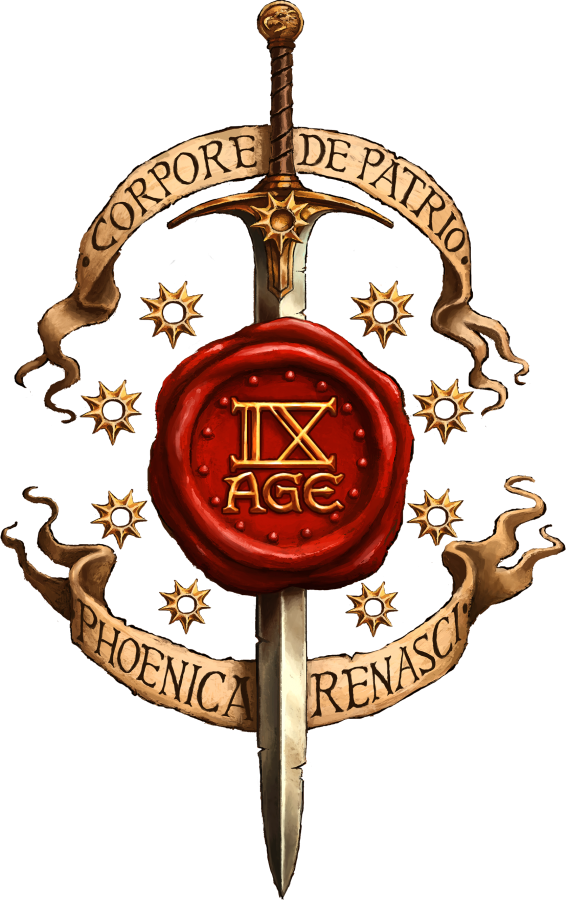
\includegraphics[height=10cm]{../Layout/pics/logo_9th.png}%
}

\vspace*{-1cm}
{\antiquefont\fontsize{50}{60}\selectfont \booktitle
\vspace{0.4cm}

\fontsize{14}{16.8}\selectfont \labels@armyrules{}

Beta v\version{} - \today{}}

\ifdef{\frenchversion}{{\fontsize{14}{16.8}\selectfont \vspace{0.2cm}\noindent\texttt{VF \frenchversion}}}{}
\vfill

\begin{tabular}{@{}m{2cm}@{\hskip 20pt}m{13cm}@{}}
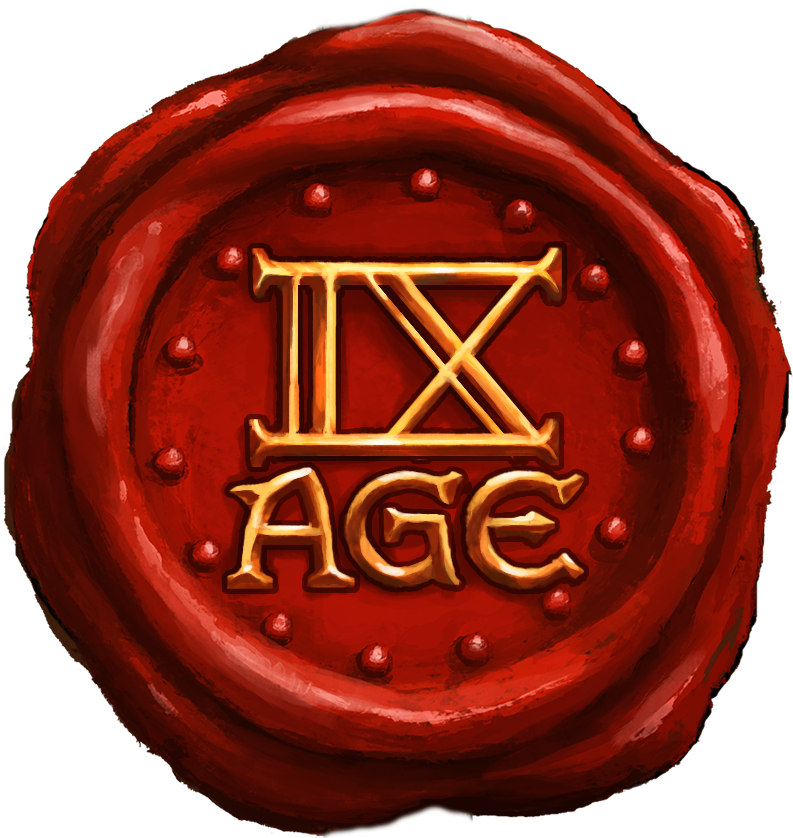
\includegraphics[width=2cm]{../Layout/pics/seal_9th.png} &
{\fontsize{10}{12}\selectfont \textcolor{black!50}{\noindent\labels@frontpagecredits}}

\ifdef{\frontpageaddstuff}{{\fontsize{10}{12}\selectfont \noindent\textcolor{black!50}{\frontpageaddstuff}}}{}

\vspace*{10pt}
\noindent{\fontsize{10}{12}\selectfont \textcolor{black!50}{\labels@license}}
\tabularnewline
\end{tabular}


\end{center}

\newpage

\thispagestyle{empty}

{\fontsize{10}{12}\selectfont

\ifdef{\labels@introduction}{\labels@introduction}{\vphantom{1pt}}
\vfill

\noindent\newrule{\labels@rulechanges}

\bigskip
\noindent \labels@latexcredit
}


\end{titlepage}

\restoregeometry

\startarmywiderules

\spaceaftersection{}

En plus des restrictions habituelles, les unités Démoniaques autres que les Démons du \truechaos{} suivent les restrictions suivantes :

\vspace*{0.2cm}
\renewcommand{\arraystretch}{2}
\begin{center}\begin{tabular}{rccc}
\hline
 & Limite de duplication & (Patrouille) & (Grande Armée) \tabularnewline
 Base & \textbf{max. 2} & max. 1 & max. 4 \tabularnewline
 Spéciale & \textbf{max. 2} & max. 1 & max. 4 \tabularnewline
 Rare & \textbf{max. 1} & max. 1 & max. 2 \tabularnewline
\hline
\end{tabular}\end{center}
\renewcommand{\arraystretch}{1.2}
\vspace*{0.2cm}

Ces restrictions sont levées pour les unités dont l'allégeance va au même Dieu Sombre que le Général. Les armées dont le Général est un Démon du \truechaos{} ignorent ces restrictions.

\armyspecialruleentry{\monotheistarmybonus}

Si toutes les unités de l'armée ont une allégeance au même Dieu Sombre, les restrictions ci-dessus ne s'appliquent plus. De plus, certaines unités obtiennent des options supplémentaires.

\closearmywiderules









\newpage
\startarmyspecialrules

\armyspecialruleentry{\daemonofthedarkgods}

Les Démons sont différents en fonction de leur allégeance à un Dieu Sombre. Chaque Dieu offre à ses démons son propre bonus, décrit ci-dessous. Toutes les figurines d'une même unité doivent appartenir au même Dieu Sombre. Les Personnages ne peuvent rejoindre que des unités démoniaques servant le même Dieu Sombre. Les figurines ne peuvent bénéficier des règles \holdyourground{} et \inspiringpresence{} que si elles proviennent d'un Démon appartenant au même Dieu Sombre qu'elles-mêmes, ou d'un Démon du \truechaos{}.

\spacebetweenalliance{}

\alliancesidepic{truechaos.png}
\hfill\alliancestartsidetext{Démon du \truechaos}
Aucun effet supplémentaire.
\allianceclosesidetext{}

\spacebetweenalliance{}

\alliancestartsidetext{Démon du \dchange}
Le Démon peut gagner une des règles suivantes, affectant les Attaques de Corps à Corps et de Tir : \divineattacks{}, \flamingattacks{} ou \hellfire{}. L'effet doit être choisi au début de chaque Manche de Corps à Corps et avant de tirer avec une unité. Toutes les figurines d'une même unité doivent choisir la même règle. Les Attaques Spéciales ne sont pas affectées. Si le Démon est un Sorcier, il peut, immédiatement après avoir lancé les dés pour générer ses sorts, choisir de tous les relancer une fois.
\allianceclosesidetext{}\hfill
\alliancesidepic{change.png}

\spacebetweenalliance{}

\alliancesidepic{wrath.png}
\hfill\alliancestartsidetext{Démon du \wrath}
Le Démon gagne +1 en Force lors de la première Manche de chaque Corps à Corps.
\allianceclosesidetext{}

\spacebetweenalliance{}

\alliancestartsidetext{Démon de la \dlust}
Le Démon gagne la règle \armourpiercing{+1}.
\allianceclosesidetext{}\hfill
\alliancesidepic{lust.png}

\spacebetweenalliance{}

\alliancesidepic{pestilence.png}
\hfill\alliancestartsidetext{Démon de la \pestilence}
Le Démon gagne les règles \poisonedattacks{} et \regeneration{5}. Les \toxicattacks{} ont un malus de -1 pour blesser le Démon.
\allianceclosesidetext{}





\newpage

\armyspecialruleentry{\aspects}

Les Démons peuvent recevoir des bonus appelés \textbf{\aspects}. L'effet d'un \aspect{} dépend du Dieu Sombre associé.

\vspace{0.2cm}
Les Personnages peuvent toujours obtenir un \aspect{}. Les Unités de Base peuvent être améliorées avec un \aspect{} si elles appartiennent au même Dieu Sombre que le Général. Certaines Unités Spéciales et Rares ne peuvent gagner un \aspect{} que dans une Armée Monothéiste où l'allégeance de toutes les figurines va au même Dieu Sombre. Plusieurs itérations d'un même \aspect{} n'apportent rien de plus que l'\aspect{} seul.

\vspace{0.5cm}
\renewcommand{\arraystretch}{2}
\begin{center}\begin{tabular}{p{2.2cm}p{12cm}}
\hline
\textbf{\dchange} & \textbf{\farseeing}\vspace{3pt}\newline
L'unité du porteur augmente de \distance{6} la portée de toutes ses Attaques de Tir qui utilise la Capacité de Tir. \tabularnewline
\textbf{\wrath} & \textbf{\onslaught}\vspace{3pt}\newline
L'unité du porteur gagne la règle \devastatingcharge{}. Les montures ne sont pas affectées. \tabularnewline
\textbf{\dlust} & \textbf{\clawedcaress}\vspace{3pt}\newline
L'unité du porteur gagne la règle \armourpiercing{+1}. \tabularnewline
\textbf{\pestilence} & \textbf{\contamination}\vspace{3pt}\newline
L'unité gagne la règle \poisonedattacks{}. Les attaques qui possèdent déjà cette règle blessent automatiquement sur un jet naturel d'un point de moins : 6+ devient 5+, et 5+ devient 4+. \tabularnewline
\hline
\end{tabular}\end{center}

\armyspecialruleentry{\supremeaspects}

Les Personnages Démoniaques peuvent être améliorés par l'\supremeaspect{} précisé dans leur profil.

\vspace{0.5cm}
\begin{center}\begin{tabular}{p{2.2cm}p{12cm}}
\hline
\textbf{\dchange} & \textbf{\powervortex}\vspace{3pt}\newline
La Force des touches des sorts de la \Pathof{} \change{} lancés par l'unité du porteur est augmentée de +1. \tabularnewline
\textbf{\wrath} & \textbf{\eternalfury}\vspace{3pt}\newline
L'unité du porteur gagne la règle \hatred{}. Les montures ne sont pas affectées. \tabularnewline
\textbf{\dlust} & \textbf{\danceofdeath}\vspace{3pt}\newline
L'unité du porteur gagne la règle \lightningreflexes{}. \tabularnewline
\textbf{\pestilence} & \textbf{\bloatedputrefaction}\vspace{3pt}\newline
L'unité du porteur gagne \regeneration{4}. \tabularnewline
\hline
\end{tabular}\end{center}
\renewcommand{\arraystretch}{1.2}

\closearmyspecialrules









\newpage
\startarmyarmoury

\vspace*{-1.0cm}
\armyspecialruleentry{Démons du \dchange}

\startitemlistonecol

\listitemonecol{\firebolts} Arme de Tir. \range{24}, \Strength{} 3, \quicktofire{}.

\enditemlistonecol

\armyspecialruleentry{Démons du \wrath}

\startitemlistonecol

\listitemonecol{\bloodsword} Arme de Corps à Corps. Type : \hw{}. Les attaques portées avec cette arme ont la règle \lethalstrike{}.

\listitemonecol{\hellblade} Arme de Corps à Corps. Type : \hw{}. Les attaques portées avec cette arme ont toujours une Force de 5. Cette valeur ne peut jamais être modifiée.

\enditemlistonecol

\armyspecialruleentry{Démons de la \dlust}

\startitemlistonecol

\listitemonecol{\barbedclaws} Arme de Corps à Corps. Type : \hw{}. Les attaques portées avec cette arme ont un bonus de +1 pour blesser au Corps à Corps.

\listitemonecol{\elusive} Les unités comprenant uniquement des figurines avec cette règle peuvent déclarer une Fuite en réponse à une charge même si elles possèdent la règle \immunetopsychology{}.

\enditemlistonecol

\armyspecialruleentry{Démons de la \pestilence}

\startitemlistonecol

\listitemonecol{\trailofmucus} Les unités ennemies n'obtiennent pas de bonus au résultat de combat pour avoir engagé le flanc ou l'arrière d'une unité comprenant au moins une figurine avec cette règle.

\enditemlistonecol

\closearmyarmoury








\toctarget{magicalitemstitle}{\startarmynewsection{Objets Démoniaques}}

\spaceaftersection{}

Les Légions Démoniaques possèdent leurs propres Objets Magiques appelés Objets Démoniaques. Les Objets Démoniaques suivent les mêmes restrictions que leurs équivalents Magiques, à l'exception que les objets limités aux porteurs appartenant à un Dieu Sombre précis peuvent être dupliqués au sein d'une même armée. Tous les Objets Magiques de l'armée doivent être choisis dans la liste ci-dessous des Objets Démoniaques, à l'exception des Bannières Magiques qui peuvent provenir des Objets Magiques du Livre de Règle. 

\begin{multicols}{2}\raggedcolumns

\subtitle{Armes Démoniaques}\vspace{5pt}

\startpricelist

\pricelistitem{\eternalsword}{50/35}Type : \hw{}. Le porteur gagne +1 en Capacité de Combat, Force et Attaque lorsqu'il est engagé au Corps à Corps.

\pricelistitem{\mortalblade}{40/30}Type : \hw{}. Les attaques portées avec cette arme ont les règles \lethalstrike{} et \multiplewounds{2}{\monster{}, \riddenmonster}.

\pricelistitem{\dissolvingtouch}{40/30}Type : \hw{}. À chaque Manche de Corps à Corps, toutes les figurines ennemies en contact avec le porteur subissent une touche avec la règle \toxicattacks{} à Initiative 10.

\pricelistitem{\lashoflust}{40/25}Démons de la \textbf{\dlust} uniquement.

Type : Arme de Tir. \range{12}, Force de l'utilisateur, \multipleshots{2D6}, \quicktofire{}. Ne peut pas être utilisé après une Marche Forcée lors du même Tour de Joueur.

\pricelistitem{\aetherwand}{40/15}Démons du \textbf{\dchange} uniquement.

Type : \hw{}. À chaque fois que le porteur lance ou dissipe un sort avec succès, lancez 1D6. Sur 4+, le porteur gagne un marqueur Charge. Pour chaque marqueur Charge, le porteur gagne +1 Attaque lorsqu'il attaque avec cette arme, de façon permanente.

\pricelistitem{\bladeofgrief}{20}Type : \hw{}. Le porteur gagne la règle \fear{} et les attaques qu'il porte avec cette arme ont la règle \divineattacks{}.

\pricelistitem{\heartseeker}{20/10}Type : \hw{}. Le porteur peut relancer tous les \result{1} pour toucher au Corps à Corps avec cette arme.

\columnbreak\vspace*{-0.1cm}
\pricelistitem{\tridentoftorment}{15}Type : \hw{}. Le porteur gagne +1 en Capacité de Combat et en Initiative quand il combat avec cette arme au Corps à Corps, et les attaques qu'il porte avec cette arme ont la règle \armourpiercing{1}.

\endpricelist

\subtitle{Talismans Démoniaques}\vspace{5pt}

\startpricelist

\pricelistitem{\nauseatingaura}{50}Démons de la \textbf{\pestilence} uniquement.

L'Initiative des unités ennemies en contact socle à socle avec le porteur passe à 1 lors de la Phase de Corps à Corps.

\pricelistitem{\shacklesofreality}{40}Le porteur gagne la règle \regeneration{4}.

\pricelistitem{\brasscollar}{35}Démons du \textbf{\wrath} uniquement.

Le porteur gagne la règle \magicresistance{3}.

\pricelistitem{\ironhide}{35}Le porteur gagne la règle \innatedefence{5}.

\pricelistitem{\veilofshadows}{35}L'unité du porteur gagne les règles \hardtarget{} et \magicresistance{1}.

\pricelistitem{\blissfulbindings}{35/25}Démons de la \textbf{\dlust} uniquement.

Les figurines ennemies attaquant le porteur voient leur caractéristique de Capacité de Combat divisée par deux, arrondie au supérieur, pour le toucher.

\pricelistitem{\weaverseye}{10}Une seule utilisation. Peut être activé lorsque le porteur rate un jet de \wardsave{}. Ce jet peut être relancé.

\endpricelist

\end{multicols}

\newpage
\begin{multicols}{2}\raggedcolumns

\subtitle{Objets Enchantés Démoniaques}\vspace{5pt}

\startpricelist

\pricelistitem{\blazingwings}{35}Démons du \textbf{\dchange} uniquement.

Le porteur gagne la règle \fly{8}.

\pricelistitem{\hornofdamnation}{35}Les unités ennemies au contact socle à socle avec le porteur ne peuvent pas bénéficier de la règle \holdyourground{}.

\pricelistitem{\obsidianhorn}{35}Une seule utilisation. Au lieu de tenter une dissipation, utilisez cet objet. Le sort est immédiatement dissipé. Cet objet ne peut être pris que si l'armée ne comprend aucun Sorcier.

\pricelistitem{\hellishcrown}{25}Le porteur gagne +1 en Commandement.

\pricelistitem{\portalgem}{20}Toutes les unités alliées à moins de \distance{6} subissent une blessure en moins lors des tests ratés d'\daemonicinstability{}.

\pricelistitem{\tokenofchange}{20}Démons du \textbf{\dchange} uniquement, \oneofakind{}.

\boundspell{3}. \changespelltwo{} (\Pathof{} \change{}).

\pricelistitem{\tokenoflust}{20}Démons de la \textbf{\dlust} uniquement, \oneofakind{}.

\boundspell{3}. \lustspellthree{} (\Pathof{} \lust{}).

\pricelistitem{\tokenofpestilence}{20}Démons de la \textbf{\pestilence} uniquement, \oneofakind{}.

\boundspell{3}. \diseasespelltwo{} (\Pathof{} \disease{}).

\pricelistitem{\blackorb}{15}Tout Sorcier ennemi qui tente de lancer un sort de la \Pathof{} \light{} subit un malus de -2 sur ses jets.

\pricelistitem{\elixirofsouls}{10}Une seule utilisation. Peut être activé au début d'une Étape des Autres Mouvements. Le porteur gagne +2 en Mouvement pour cette phase.

\endpricelist

\subtitle{Objets Cabalistiques Démoniaques}\vspace{5pt}

\startpricelist

\pricelistitem{\mirrorofchange}{40}Démons du \textbf{\dchange} uniquement.

Au début de chaque Phase de Magie alliée, le porteur peut choisir un Sorcier ennemi en ligne de vue à moins de \distance{18}. Pour la durée de cette phase, il peut lancer les sorts ne provenant pas d'\boundspell{} que connaît le Sorcier choisi à la place de ses propres sorts. Aucun sort pouvant créer des unités ou Ressusciter des figurines ne peut être lancé de cette façon.

\pricelistitem{\seventhseal}{35}Une seule utilisation. Au lieu de tenter une dissipation, utilisez cet objet. Le sort est automatiquement dissipé.

\pricelistitem{\soulboundstaff}{30}Lorsque le porteur subit un Fiasco, il compte comme ayant lancé 1 Dé de Magie de moins.

\pricelistitem{\sorcererslodestone}{30}Une seule utilisation. Immédiatement après avoir tenté un lancement ou une dissipation de sort, le porteur peut augmenter le résultat de son jet de 1D6. Cela ne compte pas comme un nouveau Dé de Pouvoir ou de Dissipation. C'est une exception à la règle des modificateurs magiques.

\pricelistitem{\scrollsoftheeighthpact}{25}Démons du \textbf{\dchange} uniquement.

Le porteur peut choisir de générer ses sorts depuis n'importe laquelle des Voies Communes, sauf la \Pathof{} \light{}. Votre choix doit toujours être indiqué sur votre liste d'armée.

\pricelistitem{\skullofcacophrax}{25/15}Le porteur génère un sort supplémentaire.

\endpricelist

\end{multicols}
\closearmynewsection








%%% START OF THE ARMYLIST - Translators shouldn't have to edit it %%%


%%% v0.99.9

\armylist

\lordstitle

\showunit{
	name={\daemonprince},
	cost=245,
	profile={< 8 9 5 6 5 4 8 5 9},
	type=\monster{},
	basesize=50x50,
	unitsize=1,
	alliance={\daemonoftruechaos},
	alliancepic={truechaos},
	allianceoptions={introsentence=\mayreplacedaemonoftruechaoswith{}, change=20, lust=\free{}, pestilence=\free{}, wrath=\free{}},
	commontype=\daemoncommonrules{},
	commonspecialrules={\daemonicinstability{},\otherworldly},
	specialrules={\stubborn},
	options={
		\magiclevelchoice{
			\magiclevel{1}=40,
			\magiclevel{2}=65,
			\magiclevel{3}=130,
			\magiclevel{4}=160,
		},
		\daemonicitems{}=\upto{}<100,
		\fly{8}=40,
		\ha{}=25,
		\platearmour{}=55,
	},
	additional={%
		\vspace*{0.3cm}\unitentryformat{\labels@magic\spacebeforecolon{}:}\newline\noindent
		\daemonprincemagic{}	
	},
}

\showunit{
	name={\weaverofchange},
	cost=540,
	profile={< 8 6 6 6 6 6 6 5 9},
	type=\monster{},
	basesize=50x100,
	unitsize=1,
	alliance={\daemonofchange},
	alliancepic={change},
	commontype=\daemoncommonrules{},
	commonspecialrules={\daemonicinstability{},\otherworldly},
	specialrules={\fly{8},\wellofpower},
	magiclevel=4,
	magicpaths={\alchemy{},\change},
	unitrules={\unitrule{\wellofpower}{\wellofpowerrule}},
	armour={\innatedefence{5}},
	options={
		\daemonicitems{}=\upto{}<100,
		\supremeaspect{}\spacebeforecolon{}: \powervortex{}=35,
	},
}

\showunit{
	name={\scourgeofwrath},
	cost=450,
	profile={< 8 10 10 6 6 6 9 7 9},
	type=\monster{},
	basesize=50x100,
	unitsize=1,
	alliance={\daemonofwrath},
	alliancepic={wrath},
	commontype=\daemoncommonrules{},
	commonspecialrules={\daemonicinstability{},\otherworldly},
	specialrules={\fly{8},\magicresistance{2}},
	armour={\ha},
	options={
		\daemonicitems{}=\upto{}<100,
		\onechoiceonly{
			\aspect\spacebeforecolon{}: \onslaught{}=10,
			\supremeaspect\spacebeforecolon{}: \eternalfury{}=30,
		},
	},
}

\showunit{
	name={\courtesanoflust},
	cost=455,
	profile={< 10 9 6 6 6 6 10 6 9},
	type=\monster{},
	basesize=50x100,
	unitsize=1,
	alliance={\daemonoflust},
	alliancepic={lust},
	commontype=\daemoncommonrules{},
	commonspecialrules={\daemonicinstability{},\otherworldly},
	specialrules={\swiftstride},
	magiclevel=2,
	magicpaths={\lust{},\shadows},
	armour={\innatedefence{5}},
	options={
		\magiclevelchoice{
			\magiclevel{3}=65,
			\magiclevel{4}=95,
		},
		\daemonicitems{}=\upto{}<100,
		\onechoiceonly{
			\aspect\spacebeforecolon{}: \clawedcaress{}=15,
			\supremeaspect\spacebeforecolon{}: \danceofdeath{}=35,
		},
	},
}

\showunit{
	name={\fatherofpestilence},
	QRSname={\fatherofpestilenceSHORT},
	cost=475,
	profile={< 6 6 3 6 7 7 4 5 9},
	type=\monster{},
	basesize=50x100,
	unitsize=1,
	alliance={\daemonofpestilence},
	alliancepic={pestilence},
	commontype=\daemoncommonrules{},
	commonspecialrules={\daemonicinstability{},\otherworldly},
	magiclevel=1,
	magicpaths={\disease{},\death},
	armour={\innatedefence{5}},
	options={
		\magiclevelchoice{
			\magiclevel{2}=25,
			\magiclevel{3}=90,
			\magiclevel{4}=120,
		},
		\daemonicitems{}=\upto{}<100,
		\onechoiceonly{
			\aspect\spacebeforecolon{}: \contamination{}=20,
			\supremeaspect\spacebeforecolon{}: \bloatedputrefaction{}=45,
		},
		\flail{}=20,
	},
}









\def\logolocalpath{../Layout/pics/logo_hero.png}%
\clearpage\toctarget{herotitle}{\bigtitle{\heroesandtheirmounts}}%
\renewcommand{\profilecategory}{\labels@heroes}%

\showunit{
	name={\harbingerofchange},
	cost=100,
	profile={< 4 3 4 3 3 2 3 2 8},
	type=\infantry{},
	basesize=25x25,
	unitsize=1,
	alliance={\daemonofchange},
	alliancepic={change},
	commontype=\daemoncommonrules{},
	commonspecialrules={\daemonicinstability{},\otherworldly},
	magiclevel=1,
	magicpaths={\alchemy{},\change},
	weapons={\firebolts},
	options={
		\bsb{}=25,
		\magiclevel{2}=25,
		\daemonicitems{}=\upto{}<50,
		\onechoiceonly{
			\aspect\spacebeforecolon{}: \farseeing{}=15,
			\supremeaspect\spacebeforecolon{}: \powervortex{}=45,
		},
	},
	mounts={
		\discofchange{}=20,
		\blazingchariot{}=100,
	},
}

\def\logolocalpath{../Layout/pics/logo_mount.png}%
\renewcommand{\profilecategory}{\labels@mounts}%

\showunit{
	name={\discofchange},
	profile={< 1 3 - 4 4 1 4 3 7},
	type=\warbeast{},
	basesize=50x50,
	alliance={\daemonofchange},
	alliancepic={change},
	commontype=\daemoncommonrules{},
	commonspecialrules={\otherworldly},
	specialrules={\fly{8}},
	armour={\mountsprotection{6}},
}

\showunit{
	notinQRS=yes,
	name={\blazingchariot},
	profile={ \chariot{}< - - - 4 4 4 - - -,
			  \skyserpent{} (2)< 1 3 - 4 - - 4 3 7},
	type=\chariot{},
	basesize=50x100,
	alliance={\daemonofchange},
	alliancepic={change},
	commontype=\daemoncommonrules{},
	commonspecialrules={\otherworldly},
	armour={\mountsprotection{6}},
	specialrules={\fly{8},\quicktofire},
	additional={%
		\def\tempweapons{\searingfirestorm{} \only{\chariot} \seeblazingchariotrareunit{}}
		\vspace*{0.3cm}\weapons{\tempweapons}
	},
}

\def\logolocalpath{../Layout/pics/logo_hero.png}%
\renewcommand{\profilecategory}{\labels@heroes}%

\newpage
\showunit{
	name={\harbingerofwrath},
	cost=95,
	profile={< 5 7 2 5 4 2 6 3 8},
	type=\infantry{},
	basesize=25x25,
	unitsize=1,
	alliance={\daemonofwrath},
	alliancepic={wrath},
	commontype=\daemoncommonrules{},
	commonspecialrules={\daemonicinstability,\otherworldly},
	specialrules={\magicresistance{1}},
	weapons={\bloodsword},
	armour={\innatedefence{6},\la},
	options={
		\bsb{}=25,
		\daemonicitems{}=\upto{}<50,
		\onechoiceonly{
			\aspect\spacebeforecolon{}: \onslaught{}=15,
			\supremeaspect\spacebeforecolon{}: \eternalfury{}=40,
		},
		\innatedefence{4}=20,
	},
	mounts={
		\crusher{}=50,
	},
}

\def\logolocalpath{../Layout/pics/logo_mount.png}%
\renewcommand{\profilecategory}{\labels@mounts}%

\showunit{
	name={\crusher},
	profile={< 7 5 - 5 4 3 2 3 7},
	type=\monstrousbeast{},
	basesize=50x75,
	alliance={\daemonofwrath},
	alliancepic={wrath},
	commontype=\daemoncommonrules{},
	commonspecialrules={\otherworldly},
	armour={\mountsprotection{6}},
	specialrules={\fear},
}

\def\logolocalpath{../Layout/pics/logo_hero.png}%
\renewcommand{\profilecategory}{\labels@heroes}%

\newpage
\showunit{
	name={\harbingeroflust},
	cost=95,
	profile={< 6 7 5 4 3 2 7 4 8},
	type=\infantry{},
	basesize=25x25,
	unitsize=1,
	alliance={\daemonoflust},
	alliancepic={lust},
	commontype=\daemoncommonrules{},
	commonspecialrules={\daemonicinstability{},\otherworldly},
	specialrules={\distracting},
	magicpaths={\lust{},\shadows},
	options={
		\bsb{}=25,
		\magiclevelchoice{
			\magiclevel{1}=40,
			\magiclevel{2}=65,
		},
		\daemonicitems{}=\upto{}<50,
		\onechoiceonly{
			\aspect\spacebeforecolon{}: \clawedcaress{}=15,
			\supremeaspect\spacebeforecolon{}: \danceofdeath{}=40,
		},
		\combatweapononechoice{
			\pw{}=5,
			\barbedclaws{}=5,
		},
	},
	mounts={
		\steedoflust{}=25,
		\sirenchariot{}=70,
	},
}

\def\logolocalpath{../Layout/pics/logo_mount.png}%
\renewcommand{\profilecategory}{\labels@mounts}%

\showunit{
	name={\steedoflust},
	profile={< 10 3 - 3 3 1 5 1 7},
	type=\warbeast{},
	basesize=25x50,
	alliance={\daemonoflust},
	alliancepic={lust},
	commontype=\daemoncommonrules{},
	commonspecialrules={\otherworldly},
	specialrules={\fastcavalry{},\elusive{},\poisonedattacks},
	armour={\mountsprotection{6}},
}

\showunit{
	notinQRS=yes,
	name={\sirenchariot},
	profile={\chariot{}< - - - 5 4 4 - - -,
			  \mountedsiren{} (1)< - 5 4 3 - - 5 2 7,
			  \steed{} (2)< 10 3 - 3 - - 5 1 7},
	type=\chariot{},
	basesize=50x100,
	alliance={\daemonoflust},
	alliancepic={lust},
	commontype=\daemoncommonrules{},
	commonspecialrules={\otherworldly},
	armour={\mountsprotection{6}},
	specialrules={\impacthits{+1},\poisonedattacks{} \only{\steed}},
}

\def\logolocalpath{../Layout/pics/logo_hero.png}%
\renewcommand{\profilecategory}{\labels@heroes}%

\newpage
\showunit{
	name={\harbingerofpestilence},
	cost=95,
	profile={< 4 5 5 5 5 2 4 3 8},
	type=\infantry{},
	basesize=25x25,
	unitsize=1,
	alliance={\daemonofpestilence},
	alliancepic={pestilence},
	commontype=\daemoncommonrules{},
	commonspecialrules={\daemonicinstability{},\otherworldly},
	magicpaths={\disease{},\death},
	options={
		\bsb{}=25,
		\magiclevelchoice{
			\magiclevel{1}=40,
			\magiclevel{2}=65,
		},
		\daemonicitems{}=\upto{}<50,
		\onechoiceonly{
			\aspect\spacebeforecolon{}: \contamination{}=40,
			\supremeaspect\spacebeforecolon{}: \bloatedputrefaction{}=40,
		},
		\combatweapononechoice{
			\flail{}=10,
			\halberd{}=15,
		},
	},
	mounts={
		\blightfly{}=40,
		\pestilentpalanquin{}=40,
	},
}

\def\logolocalpath{../Layout/pics/logo_mount.png}%
\renewcommand{\profilecategory}{\labels@mounts}%

\showunit{
	name={\blightfly},
	profile={< 1 4 3 5 5 3 2 2 7},
	type=\monstrousbeast{},
	basesize=50x75,
	alliance={\daemonofpestilence},
	alliancepic={pestilence},
	commontype=\daemoncommonrules{},
	commonspecialrules={\otherworldly},
	armour={\mountsprotection{6}},
	specialrules={\fly{6},\fear},
}

\showunit{
	name={\pestilentpalanquin},
	profile={< 4 3 3 3 3 3 3 6 7},
	type=\infantry{},
	basesize=50x50,
	alliance={\daemonofpestilence},
	alliancepic={pestilence},
	commontype=\daemoncommonrules{},
	commonspecialrules={\otherworldly},
	armour={\mountsprotection{6}},
}










\coreunitstitle

\showunit{
	name={\horrors},
	QRSname={\horror},
	cost=80,
	profile={< 4 3 3 3 3 1 3 1 7},
	type=\infantry{},
	basesize=25x25,
	unitsize=10,
	maxmodels=40,
	costpermodel=8,
	alliance={\daemonofchange},
	alliancepic={change},
	commontype=\daemoncommonrules{},
	commonspecialrules={\daemonicinstability{},\otherworldly},
	wizardconclave={\changesignature{}, \changespellone{} (\Pathof{} \change{})},
	options={
		\ifthegeneralbelongstothesamedarkgod{}\newline
			\aspect{}\spacebeforecolon{}: \farseeing{}=\permodel{}<1,
		\firebolts{}=\permodel{}<2,
	},
	commandgroup={champion=70, musician=10, banner=10, veteranstandardbearer=yessir},
}

\showunit{
	name={\slaughterers},
	QRSname={\slaughterer},
	cost=100,
	profile={< 5 5 2 4 3 1 4 1 7},
	type=\infantry{},
	basesize=25x25,
	unitsize=10,
	maxmodels=30,
	costpermodel=13,
	alliance={\daemonofwrath},
	alliancepic={wrath},
	commontype=\daemoncommonrules{},
	commonspecialrules={\daemonicinstability{},\otherworldly},
	specialrules={\magicresistance{1}},
	weapons={\bloodsword},
	options={
		\ifthegeneralbelongstothesamedarkgod{}\newline
			\aspect{}\spacebeforecolon{}: \onslaught{}=\permodel{}<1,
		\mayreplacebloodswordwithhellbladeandinnatedefence{}=\permodel{}<3,	
	},
	commandgroup={champion=10, musician=10, banner=10, veteranstandardbearer=yessir},
}

\newpage
\showunit{
	name={\sirens},
	QRSname={\siren},
	cost=130,
	profile={< 6 5 4 3 3 1 5 2 7},
	type=\infantry{},
	basesize=25x25,
	unitsize=15,
	maxmodels=35,
	costpermodel=11,
	alliance={\daemonoflust},
	alliancepic={lust},
	commontype=\daemoncommonrules{},
	commonspecialrules={\daemonicinstability{},\otherworldly},
	options={
		\ifthegeneralbelongstothesamedarkgod{}\newline
			\aspect{}\spacebeforecolon{}: \clawedcaress{}=45,
	},
	commandgroup={champion=10, musician=10, banner=10, veteranstandardbearer=yessir},
}

\showunit{
	name={\tallymen},
	QRSname={\tallyman},
	cost=100,
	profile={< 4 3 3 4 4 1 2 1 7},
	type=\infantry{},
	basesize=25x25,
	unitsize=10,
	maxmodels=30,
	costpermodel=12,
	alliance={\daemonofpestilence},
	alliancepic={pestilence},
	commontype=\daemoncommonrules{},
	commonspecialrules={\daemonicinstability{},\otherworldly},
	options={
		\onechoiceonly{
			\trailofmucus{}=\permodel{}<1,
			\parry{}=\permodel{}<1.5,
		},
		\ifthegeneralbelongstothesamedarkgod{}\newline
			\aspect{}\spacebeforecolon{}: \contamination{}=\permodel{}<2,
	},
	commandgroup={champion=10, musician=10, banner=10, veteranstandardbearer=yessir},
}









\specialunitstitle

\showunit{
	name={\igniters},
	QRSname={\igniter},
	cost=135,
	profile={< 6 3 4 4 4 1 4 2 7},
	type=\infantry{},
	basesize=25x25,
	unitsize=5,
	maxmodels=8,
	costpermodel=25,
	alliance={\daemonofchange},
	alliancepic={change},
	commontype=\daemoncommonrules{},
	commonspecialrules={\daemonicinstability{},\otherworldly},
	specialrules={\skirmisher},
	weapons={\firestorm},
	options={
		\inamonotheistarmymaytake{}
			\aspect{}\spacebeforecolon{}: \farseeing{}=\permodel{}<4,
	},
	commandgroup={champion=10},
	unitequipment={\equipmentdef{\firestorm}{\firestormrule}},
}

\showunit{
	name={\skyserpents},
	QRSname={\skyserpent},
	cost=135,
	profile={< 1 3 - 4 4 2 4 3 7},
	type=\warbeast{},
	basesize=40x40,
	unitsize=3,
	maxmodels=6,
	costpermodel=45,
	alliance={\daemonofchange},
	alliancepic={change},
	commontype=\daemoncommonrules{},
	commonspecialrules={\daemonicinstability{},\otherworldly},
	specialrules={\fly{9},\skirmisher{},\slashing},
	unitrules={\unitrule{\slashing}{\slashingrule}},
}

\showunit{
	name={\hellhounds},
	QRSname={\hellhound},
	cost=130,
	profile={< 8 5 - 4 4 2 4 2 7},
	type=\warbeast{},
	basesize=25x50,
	unitsize=5,
	maxmodels=10,
	costpermodel=23,
	alliance={\daemonofwrath},
	alliancepic={wrath},
	commontype=\daemoncommonrules{},
	commonspecialrules={\daemonicinstability{},\otherworldly},
	specialrules={\magicresistance{3}},
	armour={\innatedefence{6}},
	options={
		\ambush{}=\permodel{}<4,
		\innatedefence{4}=\permodel{}<6,
		\inamonotheistarmymaytake{}
			\aspect{}\spacebeforecolon{}: \onslaught{}=\permodel{}<3,
	},
}

\showunit{
	name={\crushercavalry},
	QRSname={\crushercavalrySING},
	cost=160,
	profile={\rider{}< 5 5 2 4 3 1 4 1 7,
			  \crusher{}< 7 5 - 5 4 3 2 3 7},
	type=\monstrouscavalry{},
	basesize=50x75,
	unitsize=3,
	maxmodels=5,
	costpermodel=60,
	alliance={\daemonofwrath},
	alliancepic={wrath},
	commontype=\daemoncommonrules{},
	commonspecialrules={\daemonicinstability{},\otherworldly},
	specialrules={\fear{},\magicresistance{1}},
	weapons={\bloodsword{} \only{\rider}},
	armour={\innatedefence{6},\mountsprotection{6}},
	options={
		\inamonotheistarmymaytake{}
			\aspect{}\spacebeforecolon{}: \onslaught{}=\permodel{}<3,
		\mayreplacebloodswordwithhellbladerideronlyandinnatedefence{}=\permodel{}<10,	
	},
	commandgroup={champion=10, musician=10, banner=10, bannerallowance=50},
}

\showunit{
	name={\mountedsirens},
	QRSname={\mountedsiren},
	cost=85,
	profile={\rider{}< 6 5 4 3 3 1 5 2 7,
			  \steedoflust{}< 10 3 - 3 3 1 5 1 7},
	type=\cavalry{},
	basesize=25x50,
	unitsize=5,
	maxmodels=15,
	costpermodel=15,
	alliance={\daemonoflust},
	alliancepic={lust},
	commontype=\daemoncommonrules{},
	commonspecialrules={\daemonicinstability{},\otherworldly},
	specialrules={\fastcavalry{},\poisonedattacks{} \only{\steed}},
	armour={\mountsprotection{6}},
	options={
		\inamonotheistarmymaytake{}
			\aspect{}\spacebeforecolon{}: \clawedcaress{}=\permodel{}<2,
		\onechoiceonly{
			\elusive{}=10,
			\barbedclaws{} \only{\rider}=\permodel{}<2,
		},
	},
	commandgroup={champion=10, musician=10, banner=10, bannerallowance=50},
}

\showunit{
	name={\sirenchariot},
	QRSname={\sirenchariot{} $^{\firstnote}$},
	cost=100,
	profile={\chariot{}< - - - 5 4 4 - - -,
			  \mountedsiren{} (2)< - 5 4 3 - - 5 2 7,
			  \steed{} (2)< 10 3 - 3 - - 5 1 7},
	type=\chariot{},
	basesize=50x100,
	unitsize=1,
	alliance={\daemonoflust},
	alliancepic={lust},
	commontype=\daemoncommonrules{},
	commonspecialrules={\daemonicinstability{},\otherworldly},
	specialrules={\impacthits{+1},\poisonedattacks{} \only{\steed}},
	armour={\mountsprotection{6}},
	options={
		\inamonotheistarmymaytake{}
			\aspect{}\spacebeforecolon{}: \clawedcaress{}=5,
		\barbedclaws{} \only{\mountedsiren}=10,
	},
}

\showunit{
	name={\clawedfiends},
	QRSname={\clawedfiend},
	cost=100,
	profile={< 10 5 - 4 4 3 5 3 7},
	type=\monstrousbeast{},
	basesize=40x40,
	unitsize=2,
	maxmodels=6,
	costpermodel=50,
	alliance={\daemonoflust},
	alliancepic={lust},
	commontype=\daemoncommonrules{},
	commonspecialrules={\daemonicinstability{},\otherworldly},
	specialrules={\fear},
	options={
		\inamonotheistarmymaytake{}
			\aspect{}\spacebeforecolon{}: \clawedcaress{}=\permodel{}<5,
		\combatweapononechoice{
			\pw{}=\permodel{}<5,
			\barbedclaws{}=\permodel{}<10,
		},
	},
}

\showunit{
	name={\pestilentbeasts},
	QRSname={\pestilentbeast},
	cost=120,
	profile={< 6 3 - 4 5 3 2 4 7},
	type=\monstrousbeast{},
	basesize=40x40,
	unitsize=2,
	maxmodels=6,
	costpermodel=60,
	alliance={\daemonofpestilence},
	alliancepic={pestilence},
	commontype=\daemoncommonrules{},
	commonspecialrules={\daemonicinstability{},\otherworldly},
	specialrules={\fear{},\regeneration{4},\trailofmucus},
	options={
		\inamonotheistarmymaytake{}
			\aspect{}\spacebeforecolon{}: \contamination{}=\permodel{}<7,
	},
}

\showunit{
	name={\plaguelings},
	cost=75,
	profile={< 4 3 3 2 3 5 2 5 7},
	type=\swarm{},
	basesize=40x40,
	unitsize=2,
	maxmodels=5,
	costpermodel=30,
	alliance={\daemonofpestilence},
	alliancepic={pestilence},
	commontype=\daemoncommonrules{},
	commonspecialrules={\daemonicinstability{},\otherworldly},
	specialrules={\scout{},\vanguard},
	options={
		\inamonotheistarmymaytake{}
			\aspect{}\spacebeforecolon{}: \contamination{}=\permodel{}<3,
	},
}

\showunit{
	name={\furies},
	QRSname={\furie},
	cost=70,
	profile={< 4 3 - 4 3 1 4 1 2},
	type=\infantry{},
	basesize=25x25,
	unitsize=5,
	maxmodels=15,
	costpermodel=10,
	alliance={\daemonoftruechaos},
	alliancepic={truechaos},
	allianceoptions={introsentence=\mayreplacedaemonoftruechaoswith{}, change=\permodel{}<2, lust=\permodel{}<2, pestilence=\permodel{}<2, wrath=\permodel{}<3},
	commontype=\daemoncommonrules{},
	commonspecialrules={\daemonicinstability{},\otherworldly},
	specialrules={\fly{10},\skirmisher},
}











\rareunitstitle

\showunit{
	name={\daemonengine},
	cost=230,
	profile={< 8 3 4 6 6 7 3 4 7},
	type=\monster{},
	basesize=150x100,
	unitsize=SPECIAL-{\textbf{(\oneofakind)} \labels@Singlemodel{}},
	alliance={\daemonoftruechaos},
	alliancepic={truechaos},
	allianceoptions={introsentence=\mayreplacedaemonoftruechaoswith{}, change=10, lust=10, pestilence=10, wrath=10},
	commontype=\daemoncommonrules{},
	commonspecialrules={\daemonicinstability{},\otherworldly},
	specialrules={\crushattack},
	armour={\innatedefence{4}},
	options={
		\pw{}=20,
	},
	additional={
		\vspace*{-0.2cm}\begin{center}\maytakeoneartilleryweapon{}\end{center}
		\setlength{\columnseprule}{0.5pt}
		\renewcommand{\columnseprulecolor}{\color{black!30}}
		\setlength{\columnsep}{1cm}
		\begin{multicols}{2}
		\raggedcolumns		

		\begin{center}{\largerfontsize\antiquefont\hellishreaper{} (\pts{20})}\end{center}
		
		\noindent\hellishreaperrule{}
		
		\vspace*{10pt}\begin{center}{\largerfontsize\antiquefont\hellishbolt{} (\pts{35})}\end{center}
		
		\noindent\hellishboltrule{}
		
		\vspace*{\fill}\columnbreak
		
		\begin{center}{\largerfontsize\antiquefont\hellishbombard{} (\pts{40})}\end{center}
		
		\noindent\hellishbombardrule{}
		
		\vspace*{10pt}\begin{center}{\largerfontsize\antiquefont\hellishbreath{} (\pts{40})}\end{center}
		
		\noindent\hellishbreathrule{}
		
		\vspace*{\fill}\end{multicols}
		\setlength{\columnseprule}{0pt}
	},
}

\showunit{
	name={\blazingchariot},
	QRSname={\blazingchariot{} $^{\secondnote}$},
	cost=135,
	profile={ \chariot{}< - - - 4 4 4 - - -,
			  \exaltedigniter{} (1)< - 4 4 4 - - 4 3 7,
			  \skyserpent{} (2)< 1 3 - 4 - - 4 3 7},
	type=\chariot{},
	basesize=50x100,
	unitsize=1,
	alliance={\daemonofchange},
	alliancepic={change},
	armour={\mountsprotection{6}},
	commontype=\daemoncommonrules{},
	commonspecialrules={\daemonicinstability{},\otherworldly},
	specialrules={\fly{8},\quicktofire},
	weapons={\searingfirestorm{} \only{\chariot}},
	options={
		\inamonotheistarmymaytake{}
			\aspect{}\spacebeforecolon{}: \farseeing{}=10,
	},
	additional={%
		\def\tempunitequipment{\equipmentdef{\searingfirestorm}{\searingfirestormrule}}
		\unitequipment{\tempunitequipment}
	},
}

\showunit{
	name={\bloodchariot},
	cost=165,
	profile={ \chariot{}< - - - 5 5 4 - - -,
			  \slaughterer{} (2)< - 5 3 4 - - 4 1 7,
			  \crusher{} (1)< 7 5 - 5 - - 2 3 7},
	type=\chariot{},
	basesize=50x100,
	unitsize=1,
	alliance={\daemonofwrath},
	alliancepic={wrath},
	commontype=\daemoncommonrules{},
	commonspecialrules={\daemonicinstability{},\otherworldly},
	specialrules={\fear{},\impacthits{+1},\magicresistance{1}},
	weapons={\bloodsword{} \only{\slaughterer}},
	armour={\innatedefence{4},\mountsprotection{6}},
	options={
		\inamonotheistarmymaytake{}
			\aspect{}\spacebeforecolon{}: \onslaught{}=10,
	},
	additional={
		\begin{center}\musttakeoneofthefollowingNOC{}\end{center}
		\setlength{\columnseprule}{0.5pt}
		\renewcommand{\columnseprulecolor}{\color{black!30}}
		\setlength{\columnsep}{1cm}
		\vspace*{-0.2cm}\begin{multicols}{2}
		\raggedcolumns		

		\begin{center}{\largerfontsize\antiquefont\incinerator{} (\free)}\end{center}
		
		\noindent\incineratorrule{}
		
		\vspace*{\fill}\columnbreak
		\begin{center}{\largerfontsize\antiquefont\brasscannon{} (\free)}\end{center}
		
		\noindent\brasscannonrule{}
	
		\vspace*{\fill}
		\end{multicols}
		\setlength{\columnseprule}{0pt}
	},
}

\showunit{
	name={\altarofslaughter},
	cost=180,
	profile={ \chariot{}< - - - 5 6 4 - - -,
			  \doombringer{} (1)< - 5 3 4 - - 4 2 7,
			  \slaughterer{} (2)< - 5 3 4 - - 4 1 7,
			  \crusher{} (1)< 7 5 - 5 - - 2 3 7},
	type=\chariot{},
	basesize=50x100,
	unitsize=SPECIAL-{\textbf{(\oneofakind)} \labels@Singlemodel{}},
	alliance={\daemonofwrath},
	alliancepic={wrath},
	commontype=\daemoncommonrules{},
	commonspecialrules={\daemonicinstability{},\otherworldly},
	specialrules={\fear{},\impacthits{+1},\magicresistance{2}},
	weapons={\bloodsword{} \only{\crew}},
	armour={\innatedefence{4},\mountsprotection{6}},
	unitrules={\unitrule{\bloodfeast}{\bloodfeastrule}},
	options={
		\bloodfeast{}=15,
		\inamonotheistarmymaytake{}
			\aspect{}\spacebeforecolon{}: \onslaught{}=15,
	},
}

\showunit{
	name={\shrineoftemptation},
	cost=180,
	profile={ \chariot{}< - - - 5 5 5 - - -,
			  \temptress{} (1)< - 5 5 3 - - 5 4 7,
			  \mountedsiren{} (3)< - 5 4 3 - - 5 2 7,
			  \steed{} (4)< 10 3 - 3 - - 5 1 7},
	type=\chariot{},
	basesize=100x150,
	unitsize=1,
	alliance={\daemonoflust},
	alliancepic={lust},
	commontype=\daemoncommonrules{},
	commonspecialrules={\daemonicinstability{},\otherworldly},
	specialrules={\impacthits{+3},\poisonedattacks{} \only{\steed}},
	armour={\mountsprotection{6}},
	unitrules={\unitrule{\auraofecstasy}{\auraofecstasyrule}},
	options={
		\auraofecstasy{}=15,
		\inamonotheistarmymaytake{}
			\aspect{}\spacebeforecolon{}: \clawedcaress{}=15,
		\lashoflust{} \only{\temptress}=15,
		\barbedclaws{} \only{\crew}=20,
	},
}

\showunit{
	name={\carnalchariot},
	cost=110,
	profile={ \chariot{}< - - - 4 4 4 - - -,
			  \oracle{} (1)< - 5 4 3 - - 5 2 7,
			  \mountedsiren{} (2)< - 5 4 3 - - 5 2 7,
			  \steed{} (2)< 10 3 - 3 - - 5 1 7},
	type=\chariot{},
	basesize=100x150,
	unitsize=1,
	alliance={\daemonoflust},
	alliancepic={lust},
	commontype=\daemoncommonrules{},
	commonspecialrules={\daemonicinstability{},\otherworldly},
	armour={\mountsprotection{6}},
	options={
		\inamonotheistarmymaytake{}
			\aspect{}\spacebeforecolon{}: \clawedcaress{}=10,
		\barbedclaws{} \only{\crew}=15,
	},
	additional={%
		\def\tempspecialrules{\impacthits{+1},\poisonedattacks{} \only{\steed},\soulreaper}
		\specialrules{\tempspecialrules}
		
		\def\tempunitrules{\unitrule{\soulreaper}{\soulreaperrule}}
		\vspace*{0.15cm}\unitrules{\tempunitrules}
	},
}

\showunit{
	name={\blightflies},
	QRSname={\blightfly},
	cost=170,
	profile={\rider{}< 4 4 4 4 4 1 2 2 7,
			  \blightfly{}< 1 4 - 5 5 3 2 2 7},
	type=\monstrouscavalry{},
	basesize=50x75,
	unitsize=3,
	maxmodels=5,
	costpermodel=70,
	alliance={\daemonofpestilence},
	alliancepic={pestilence},
	commontype=\daemoncommonrules{},
	commonspecialrules={\daemonicinstability{},\otherworldly},
	armour={\mountsprotection{6}},
	specialrules={\fear{},\fly{6}},
	options={
		\inamonotheistarmymaytake{}
			\aspect{}\spacebeforecolon{}: \contamination{}=\permodel{}<5,
	},
	commandgroup={champion=10, musician=10, banner=10, bannerallowance=50},
}




%%% Quick Reference Sheet - AB_qrs.tex is automatic and shouldn't be edited %%%

\quickrefsheettitle

% Script to automatically draw the Quick Ref Sheet

\renewcommand{\arraystretch}{1.2}

\providebool{QRSbool}

\providebool{whiterow}

\newcommand{\QRSrowcolor}{\ifbool{whiterow}{\global\boolfalse{whiterow}}{\rowcolor{black!10}\global\booltrue{whiterow}}}

\newcommand{\QRSstarttab}[1]{%
	\noindent%
	\setlength{\tabcolsep}{2pt}%
	\begin{tabular}{@{}cp{3.2cm}M{\profilecellsize}@{}M{\profilecellsize}@{}M{\profilecellsize}@{}M{\profilecellsize}@{}M{\profilecellsize}@{}M{\profilecellsize}@{}M{\profilecellsize}@{}M{\profilecellsize}@{}M{\profilecellsize}}%

	& \antiquefont\large{\textbf{#1}} & \textbf{\labels@M} & \textbf{\labels@WS} & \textbf{\labels@BS} & \textbf{\labels@S} & \textbf{\labels@T} & \textbf{\labels@W} & \textbf{\labels@I} & \textbf{\labels@A} & \textbf{\labels@Ld}%
}%

\newcommand{\QRSclosetab}{\end{tabular}\bigskip}%

\newcommand{\QRSprintline}[4]{%
	\tabularnewline%
	\ifnumequal{\rowmulti}{1}{\QRSrowcolor}{}%
	\DTLifeq*{\rowcategory}{\labels@lords}{\antiquefont\bfseries \labels@lordsInitial}{}%
	\DTLifeq*{\rowcategory}{\labels@heroes}{\antiquefont\bfseries \labels@heroesInitial}{}%
	\DTLifeq*{\rowcategory}{\labels@coreunits}{\antiquefont\bfseries \labels@coreunitsInitial}{}%
	\DTLifeq*{\rowcategory}{\labels@specialunits}{\antiquefont\bfseries \labels@specialunitsInitial}{}%
	\DTLifeq*{\rowcategory}{\labels@rareunits}{\antiquefont\bfseries \labels@rareunitsInitial}{}%
	\DTLifeq*{\rowcategory}{\labels@mounts}{\antiquefont\bfseries \labels@mountsInitial}{}%
	&%
	\ifnumequal{\rowmulti}{1}{%no Multiprofile
		\rowname%
		\expandafter\parselist\expandafter{\rowprofile}{\locallists@profileslist}%
		\forlistloop{\QRSmonoprofile}{\locallists@profileslist}%
	}{% Multiprofile
		\rowname &&&&&&&&&%
		\expandafter\parselist\expandafter{\rowprofile}{\locallists@profileslist}%
		\forlistloop{\QRSmultiprofile}{\locallists@profileslist}%
	}%
}

\newcommand{\QRSmultiprofile}[1]{%
	\tabularnewline%
	\QRSrowcolor{}&%
	\splitatinf{#1}\local@unitname\local@unitprofile%
	- \local@unitname \expandafter\caraclist\expandafter{\local@unitprofile}%
}%

\newcommand{\QRSmonoprofile}[1]{%
	\splitatinf{#1}\local@unitname\local@unitprofile%
	\expandafter\caraclist\expandafter{\local@unitprofile}%
}%

\newcommand{\QRSprinttab}[1]{%
	\global\booltrue{whiterow}%
	\DTLforeach*[#1]%
	{profiles}{\rowname=name, \rowtrooptype=trooptype, \rowcategory=category, \rowprofile=profile, \rowmulti=multipleprofile}{%
      		\QRSprintline{\rowname}{\rowcategory}{\rowprofile}{\rowmulti}%
	}%
}%

\providebool{QRSisempty}
\global\boolfalse{QRSisempty}%

\newcommand{\QRScheckifempty}[1]{%
	\global\booltrue{QRSisempty}%
	\DTLforeach*[#1]%
	{profiles}{\rowname=name, \rowtrooptype=trooptype, \rowcategory=category, \rowprofile=profile, \rowmulti=multipleprofile}{%
		\global\boolfalse{QRSisempty}\dtlbreak%
	}%
}%

\newcommand{\QRSifnotempty}[1]{%
	\ifbool{QRSisempty}{}{#1}%
}%

\begin{center}
{\antiquefont\bfseries \labels@lordsInitial}\spacebeforecolon{}: \labels@lords{} - %
{\antiquefont\bfseries \labels@heroesInitial}\spacebeforecolon{}: \labels@heroes{} - %
{\antiquefont\bfseries \labels@coreunitsInitial}\spacebeforecolon{}: \labels@coreunits{} - %
{\antiquefont\bfseries \labels@specialunitsInitial}\spacebeforecolon{}: \labels@specialunits{} - %
{\antiquefont\bfseries \labels@rareunitsInitial}\spacebeforecolon{}: \labels@rareunits{} - %
{\antiquefont\bfseries \labels@mountsInitial}\spacebeforecolon{}: \labels@mounts{}%
\end{center}

\begin{multicols}{2}

\QRScheckifempty{%
	\DTLiseq{\rowcategory}{\labels@lords}\or\DTLiseq{\rowcategory}{\labels@heroes}%
}%
\QRSifnotempty{%
	\QRSstarttab{\characters}%
	\QRSprinttab{%
		\DTLiseq{\rowcategory}{\labels@lords}\or\DTLiseq{\rowcategory}{\labels@heroes}%
	}%
	\QRSclosetab{}%
}%

\QRScheckifempty{%
	\DTLiseq{\rowtrooptype}{\infantry}\and\not\DTLiseq{\rowcategory}{\labels@heroes}\and\not\DTLiseq{\rowcategory}{\labels@lords}%
}%
\QRSifnotempty{%
	\QRSstarttab{\infantry}%
	\QRSprinttab{%
		\DTLiseq{\rowtrooptype}{\infantry}\and\not\DTLiseq{\rowcategory}{\labels@heroes}\and\not\DTLiseq{\rowcategory}{\labels@lords}%
	}% 
	\QRSclosetab{}%
}% 

\QRScheckifempty{%
	\DTLiseq{\rowtrooptype}{\monstrousinfantry}\and\not\DTLiseq{\rowcategory}{\labels@heroes}\and\not\DTLiseq{\rowcategory}{\labels@lords}%
}%
\QRSifnotempty{%
	\QRSstarttab{\monstrousinfantry}%
	\QRSprinttab{%
		\DTLiseq{\rowtrooptype}{\monstrousinfantry}\and\not\DTLiseq{\rowcategory}{\labels@heroes}\and\not\DTLiseq{\rowcategory}{\labels@lords}%
	}% 
	\QRSclosetab{}%
}% 

\QRScheckifempty{%
	\DTLiseq{\rowtrooptype}{\warbeast}\and\not\DTLiseq{\rowcategory}{\labels@heroes}\and\not\DTLiseq{\rowcategory}{\labels@lords}%
}%
\QRSifnotempty{%
	\QRSstarttab{\warbeasts}%
	\QRSprinttab{%
		\DTLiseq{\rowtrooptype}{\warbeast}\and\not\DTLiseq{\rowcategory}{\labels@heroes}\and\not\DTLiseq{\rowcategory}{\labels@lords}%
	}% 
	\QRSclosetab{}%
}% 

\QRScheckifempty{%
	\DTLiseq{\rowtrooptype}{\monstrousbeast}\and\not\DTLiseq{\rowcategory}{\labels@heroes}\and\not\DTLiseq{\rowcategory}{\labels@lords}%
}%
\QRSifnotempty{%
	\QRSstarttab{\monstrousbeasts}%
	\QRSprinttab{%
		\DTLiseq{\rowtrooptype}{\monstrousbeast}\and\not\DTLiseq{\rowcategory}{\labels@heroes}\and\not\DTLiseq{\rowcategory}{\labels@lords}%
	}% 
	\QRSclosetab{}%
}% 

\QRScheckifempty{%
	\DTLiseq{\rowtrooptype}{\cavalry}\and\not\DTLiseq{\rowcategory}{\labels@heroes}\and\not\DTLiseq{\rowcategory}{\labels@lords}%
}%
\QRSifnotempty{%
	\QRSstarttab{\cavalry}%
	\QRSprinttab{%
		\DTLiseq{\rowtrooptype}{\cavalry}\and\not\DTLiseq{\rowcategory}{\labels@heroes}\and\not\DTLiseq{\rowcategory}{\labels@lords}%
	}%
	\QRSclosetab{}%
}% 

\QRScheckifempty{%
	\DTLiseq{\rowtrooptype}{\monstrouscavalry}\and\not\DTLiseq{\rowcategory}{\labels@heroes}\and\not\DTLiseq{\rowcategory}{\labels@lords}%
}%
\QRSifnotempty{%
	\QRSstarttab{\monstrouscavalry}%
	\QRSprinttab{%
		\DTLiseq{\rowtrooptype}{\monstrouscavalry}\and\not\DTLiseq{\rowcategory}{\labels@heroes}\and\not\DTLiseq{\rowcategory}{\labels@lords}%
	}%
	\QRSclosetab{}%
}% 

\QRScheckifempty{%
	\DTLiseq{\rowtrooptype}{\chariot}\and\not\DTLiseq{\rowcategory}{\labels@heroes}\and\not\DTLiseq{\rowcategory}{\labels@lords}%
}%
\QRSifnotempty{%
	\QRSstarttab{\chariots}%
	\QRSprinttab{%
		\DTLiseq{\rowtrooptype}{\chariot}\and\not\DTLiseq{\rowcategory}{\labels@heroes}\and\not\DTLiseq{\rowcategory}{\labels@lords}%
	}%
	\QRSclosetab{}%
}% 

\QRScheckifempty{%
	\DTLiseq{\rowtrooptype}{\monster}\and\not\DTLiseq{\rowcategory}{\labels@heroes}\and\not\DTLiseq{\rowcategory}{\labels@lords}%
}%
\QRSifnotempty{%
	\QRSstarttab{\monsters}%
	\QRSprinttab{%
		\DTLiseq{\rowtrooptype}{\monster}\and\not\DTLiseq{\rowcategory}{\labels@heroes}\and\not\DTLiseq{\rowcategory}{\labels@lords}%
	}%
	\QRSclosetab{}%
}% 

\QRScheckifempty{%
	\DTLiseq{\rowtrooptype}{\riddenmonster}\and\not\DTLiseq{\rowcategory}{\labels@heroes}\and\not\DTLiseq{\rowcategory}{\labels@lords}%
}%
\QRSifnotempty{%
	\QRSstarttab{\riddenmonsters}%
	\QRSprinttab{%
		\DTLiseq{\rowtrooptype}{\riddenmonster}\and\not\DTLiseq{\rowcategory}{\labels@heroes}\and\not\DTLiseq{\rowcategory}{\labels@lords}%
	}%
	\QRSclosetab{}%
}% 

\QRScheckifempty{%
	\DTLiseq{\rowtrooptype}{\swarm}\and\not\DTLiseq{\rowcategory}{\labels@heroes}\and\not\DTLiseq{\rowcategory}{\labels@lords}%
}%
\QRSifnotempty{%
	\QRSstarttab{\swarms}%
	\QRSprinttab{%
		\DTLiseq{\rowtrooptype}{\swarm}\and\not\DTLiseq{\rowcategory}{\labels@heroes}\and\not\DTLiseq{\rowcategory}{\labels@lords}%
	}%
	\QRSclosetab{}%
}% 

\end{multicols}
\bigskip
\begin{center}
\noindent{\antiquefont\Largefontsize\textbf{Armes de Tir des Démons}}
\medskip

\rowcolors{1}{white}{black!10}
\noindent\begin{tabular}{lcccccc}
\textbf{Nom} & \textbf{Artillerie} & \textbf{Portée} & \textbf{\labels@S{}} & \textbf{\multipleshots{}} & \textbf{\multiplewounds{}} & \textbf{\armourpiercing{}} \tabularnewline
\firebolts{} & - & \distance{24} & 3 & - & - & - \tabularnewline
\firestorm{} & - & \distance{18} & 4 & 1D3 & - & - \tabularnewline
\searingfirestorm{} (1) & \boltthrower{} & \distance{24} & 4 + 1D3 & - & 1D3 & 6 \tabularnewline
\searingfirestorm{} (2) & \volleygun{} & \distance{24} & 2 + 1D3 & 6 & - & - \tabularnewline
\incinerator{} & \flamethrower{} & \distance{8} & 4 & - & - & - \tabularnewline
\brasscannon{} & \cannon{} (\distance{1D6}) & \distance{48} & 10 & - & \ordnance{} & 2 \tabularnewline
\hellishreaper{} & \volleygun{} & \distance{12} & 4 & 2D6 & - & 3 \tabularnewline
\hellishbreath{} & \flamethrower{} & \distance{8} & 4 & - & - & - \tabularnewline
\hellishbombard{} & \catapult{} (\distance{3}) & \distance{12-60} & 3 [9] & - & [\ordnance{}] & - \tabularnewline
\hellishbolt{} & \boltthrower{} & \distance{48} & 6 & - & 1D3 & 6 \tabularnewline
\end{tabular}
\end{center}

\renewcommand{\firstnote}{2}
\renewcommand{\secondnote}{1}
\renewcommand{\QRSnote}{%
\noindent$^{\secondnote}$ Pas d'\igniter{} quand il sert de monture.

\noindent$^{\firstnote}$ Un membre d'équipage de moins quand il sert de monture.
}

\clearpage\toctarget{QRSmonotitle}{\bigtitle{Fiche de référence monothéiste}}\vspace*{0.4cm}


\renewcommand{\QRSprinttab}[1]{%
	\global\booltrue{whiterow}%
	\DTLforeach*[#1]%
	{profiles}{\rowname=name, \rowtrooptype=trooptype, \rowcategory=category, \rowprofile=profile, \rowmulti=multipleprofile, \rowalliancepic=alliancepic}{%
      		\QRSprintline{\rowname}{\rowcategory}{\rowprofile}{\rowmulti}%
	}%
}%

\renewcommand{\QRScheckifempty}[1]{%
	\global\booltrue{QRSisempty}%
	\DTLforeach*[#1]%
	{profiles}{\rowname=name, \rowtrooptype=trooptype, \rowcategory=category, \rowprofile=profile, \rowmulti=multipleprofile, \rowalliancepic=alliancepic}{%
		\global\boolfalse{QRSisempty}\dtlbreak%
	}%
}%

\begin{center}
{\antiquefont\bfseries \labels@lordsInitial}\spacebeforecolon{}: \labels@lords{} - %
{\antiquefont\bfseries \labels@heroesInitial}\spacebeforecolon{}: \labels@heroes{} - %
{\antiquefont\bfseries \labels@coreunitsInitial}\spacebeforecolon{}: \labels@coreunits{} - %
{\antiquefont\bfseries \labels@specialunitsInitial}\spacebeforecolon{}: \labels@specialunits{} - %
{\antiquefont\bfseries \labels@rareunitsInitial}\spacebeforecolon{}: \labels@rareunits{} - %
{\antiquefont\bfseries \labels@mountsInitial}\spacebeforecolon{}: \labels@charactermounts{} \labels@only{}%
\end{center}

\begin{multicols}{2}\raggedcolumns

\begin{center}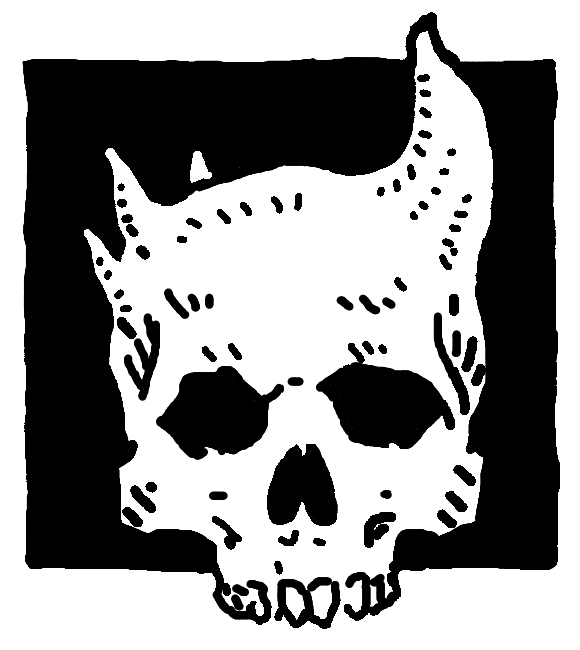
\includegraphics[width=1.2cm]{pics/truechaos.png}\end{center}

\QRScheckifempty{%
	\DTLiseq{\rowalliancepic}{truechaos}%
}%
\QRSifnotempty{%
	\QRSstarttab{\truechaos}%
	\QRSprinttab{%
		\DTLiseq{\rowalliancepic}{truechaos}%
	}%
	\QRSclosetab{}%
}%

\begin{center}
\includegraphics[width=1.2cm]{pics/change.png}\end{center}

\QRScheckifempty{%
	\DTLiseq{\rowalliancepic}{change}%
}%
\QRSifnotempty{%
	\QRSstarttab{\dchange}%
	\QRSprinttab{%
		\DTLiseq{\rowalliancepic}{change}%
	}%
	\QRSclosetab{}%
}%

\begin{center}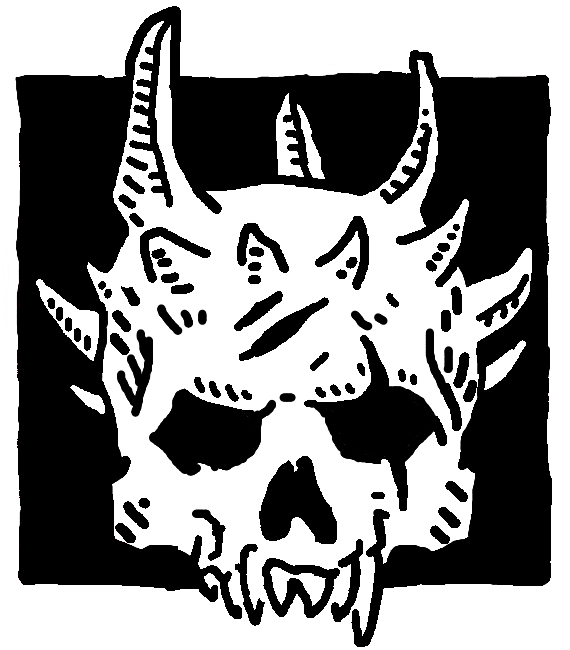
\includegraphics[width=1.2cm]{pics/wrath.png}\end{center}

\QRScheckifempty{%
	\DTLiseq{\rowalliancepic}{wrath}%
}%
\QRSifnotempty{%
	\QRSstarttab{\wrath}%
	\QRSprinttab{%
		\DTLiseq{\rowalliancepic}{wrath}%
	}%
	\QRSclosetab{}%
}%

\begin{center}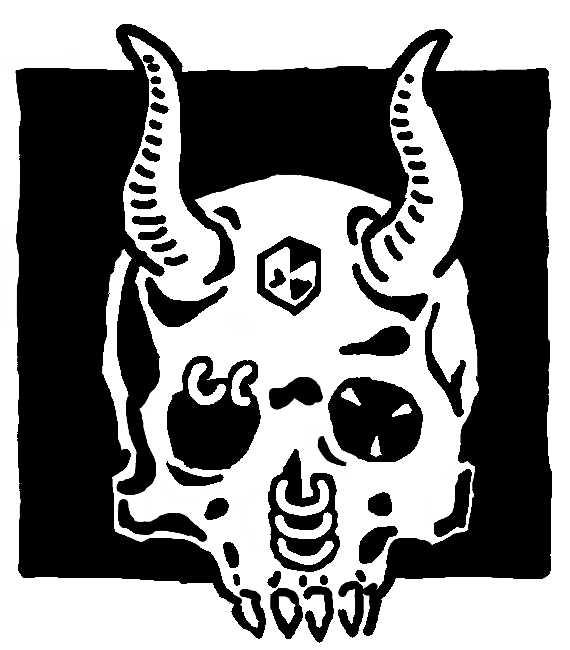
\includegraphics[width=1.2cm]{pics/lust.png}\end{center}

\QRScheckifempty{%
	\DTLiseq{\rowalliancepic}{lust}%
}%
\QRSifnotempty{%
	\QRSstarttab{\dlust}%
	\QRSprinttab{%
		\DTLiseq{\rowalliancepic}{lust}%
	}%
	\QRSclosetab{}%
}%

\begin{center}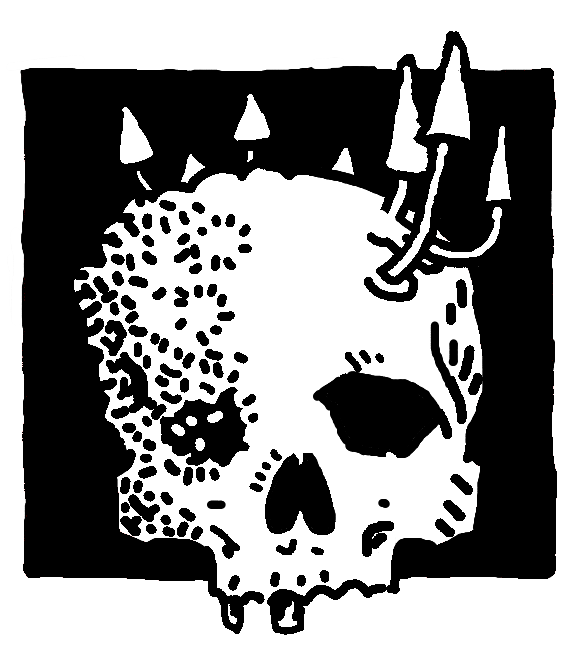
\includegraphics[width=1.2cm]{pics/pestilence.png}\end{center}

\QRScheckifempty{%
	\DTLiseq{\rowalliancepic}{pestilence}%
}%
\QRSifnotempty{%
	\QRSstarttab{\pestilence}%
	\QRSprinttab{%
		\DTLiseq{\rowalliancepic}{pestilence}%
	}%
	\QRSclosetab{}%
}%

\ifdef{\QRSnote}{\QRSnote}{}

\end{multicols}

\restoregeometry

\end{document}
